\section{Fundamentos físicos}


\subsection{Radiación electromagnética}
\begin{frame}{\secname : \subsecname}
  \begin{figure}
    \centering
    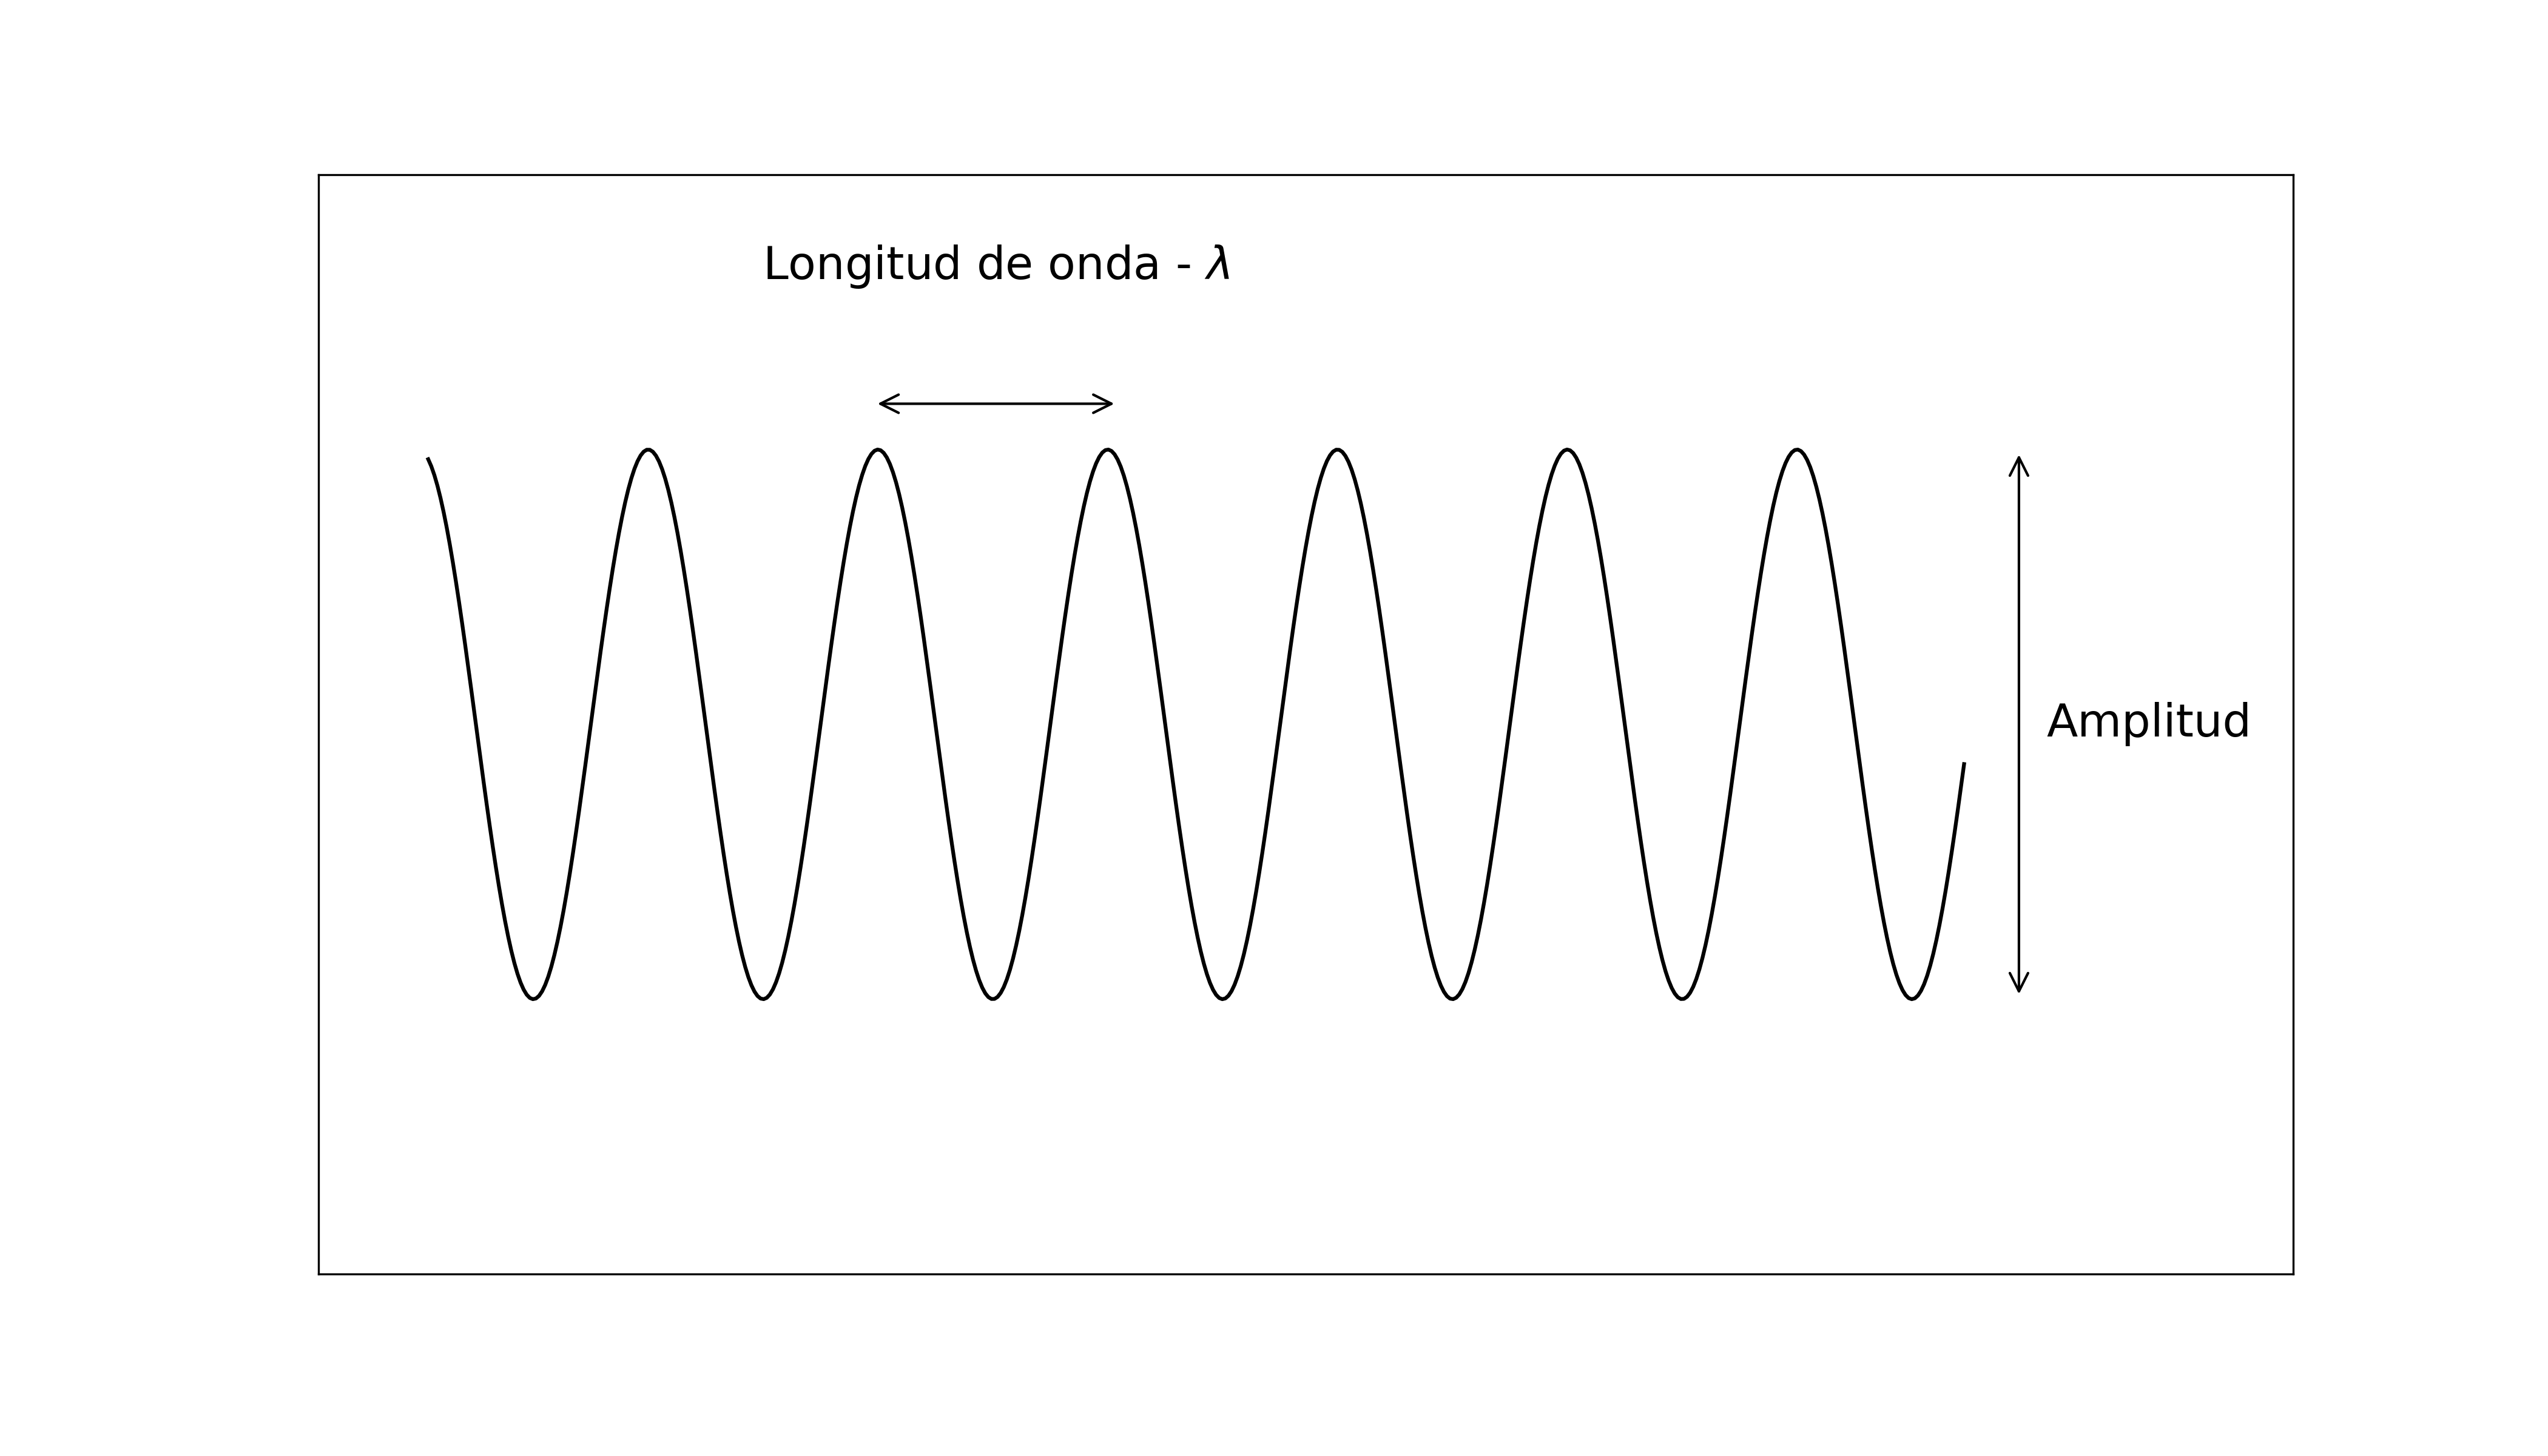
\includegraphics[width=0.8\textwidth]{fig:wavek.png}
    \caption{Radiación electromagnética. Una onda que se propaga en el espacio.}
    \label{}
  \end{figure}
\end{frame}
%--- Next Frame ---%

\begin{frame}{\secname : \subsecname}
  \begin{figure}
    \centering
    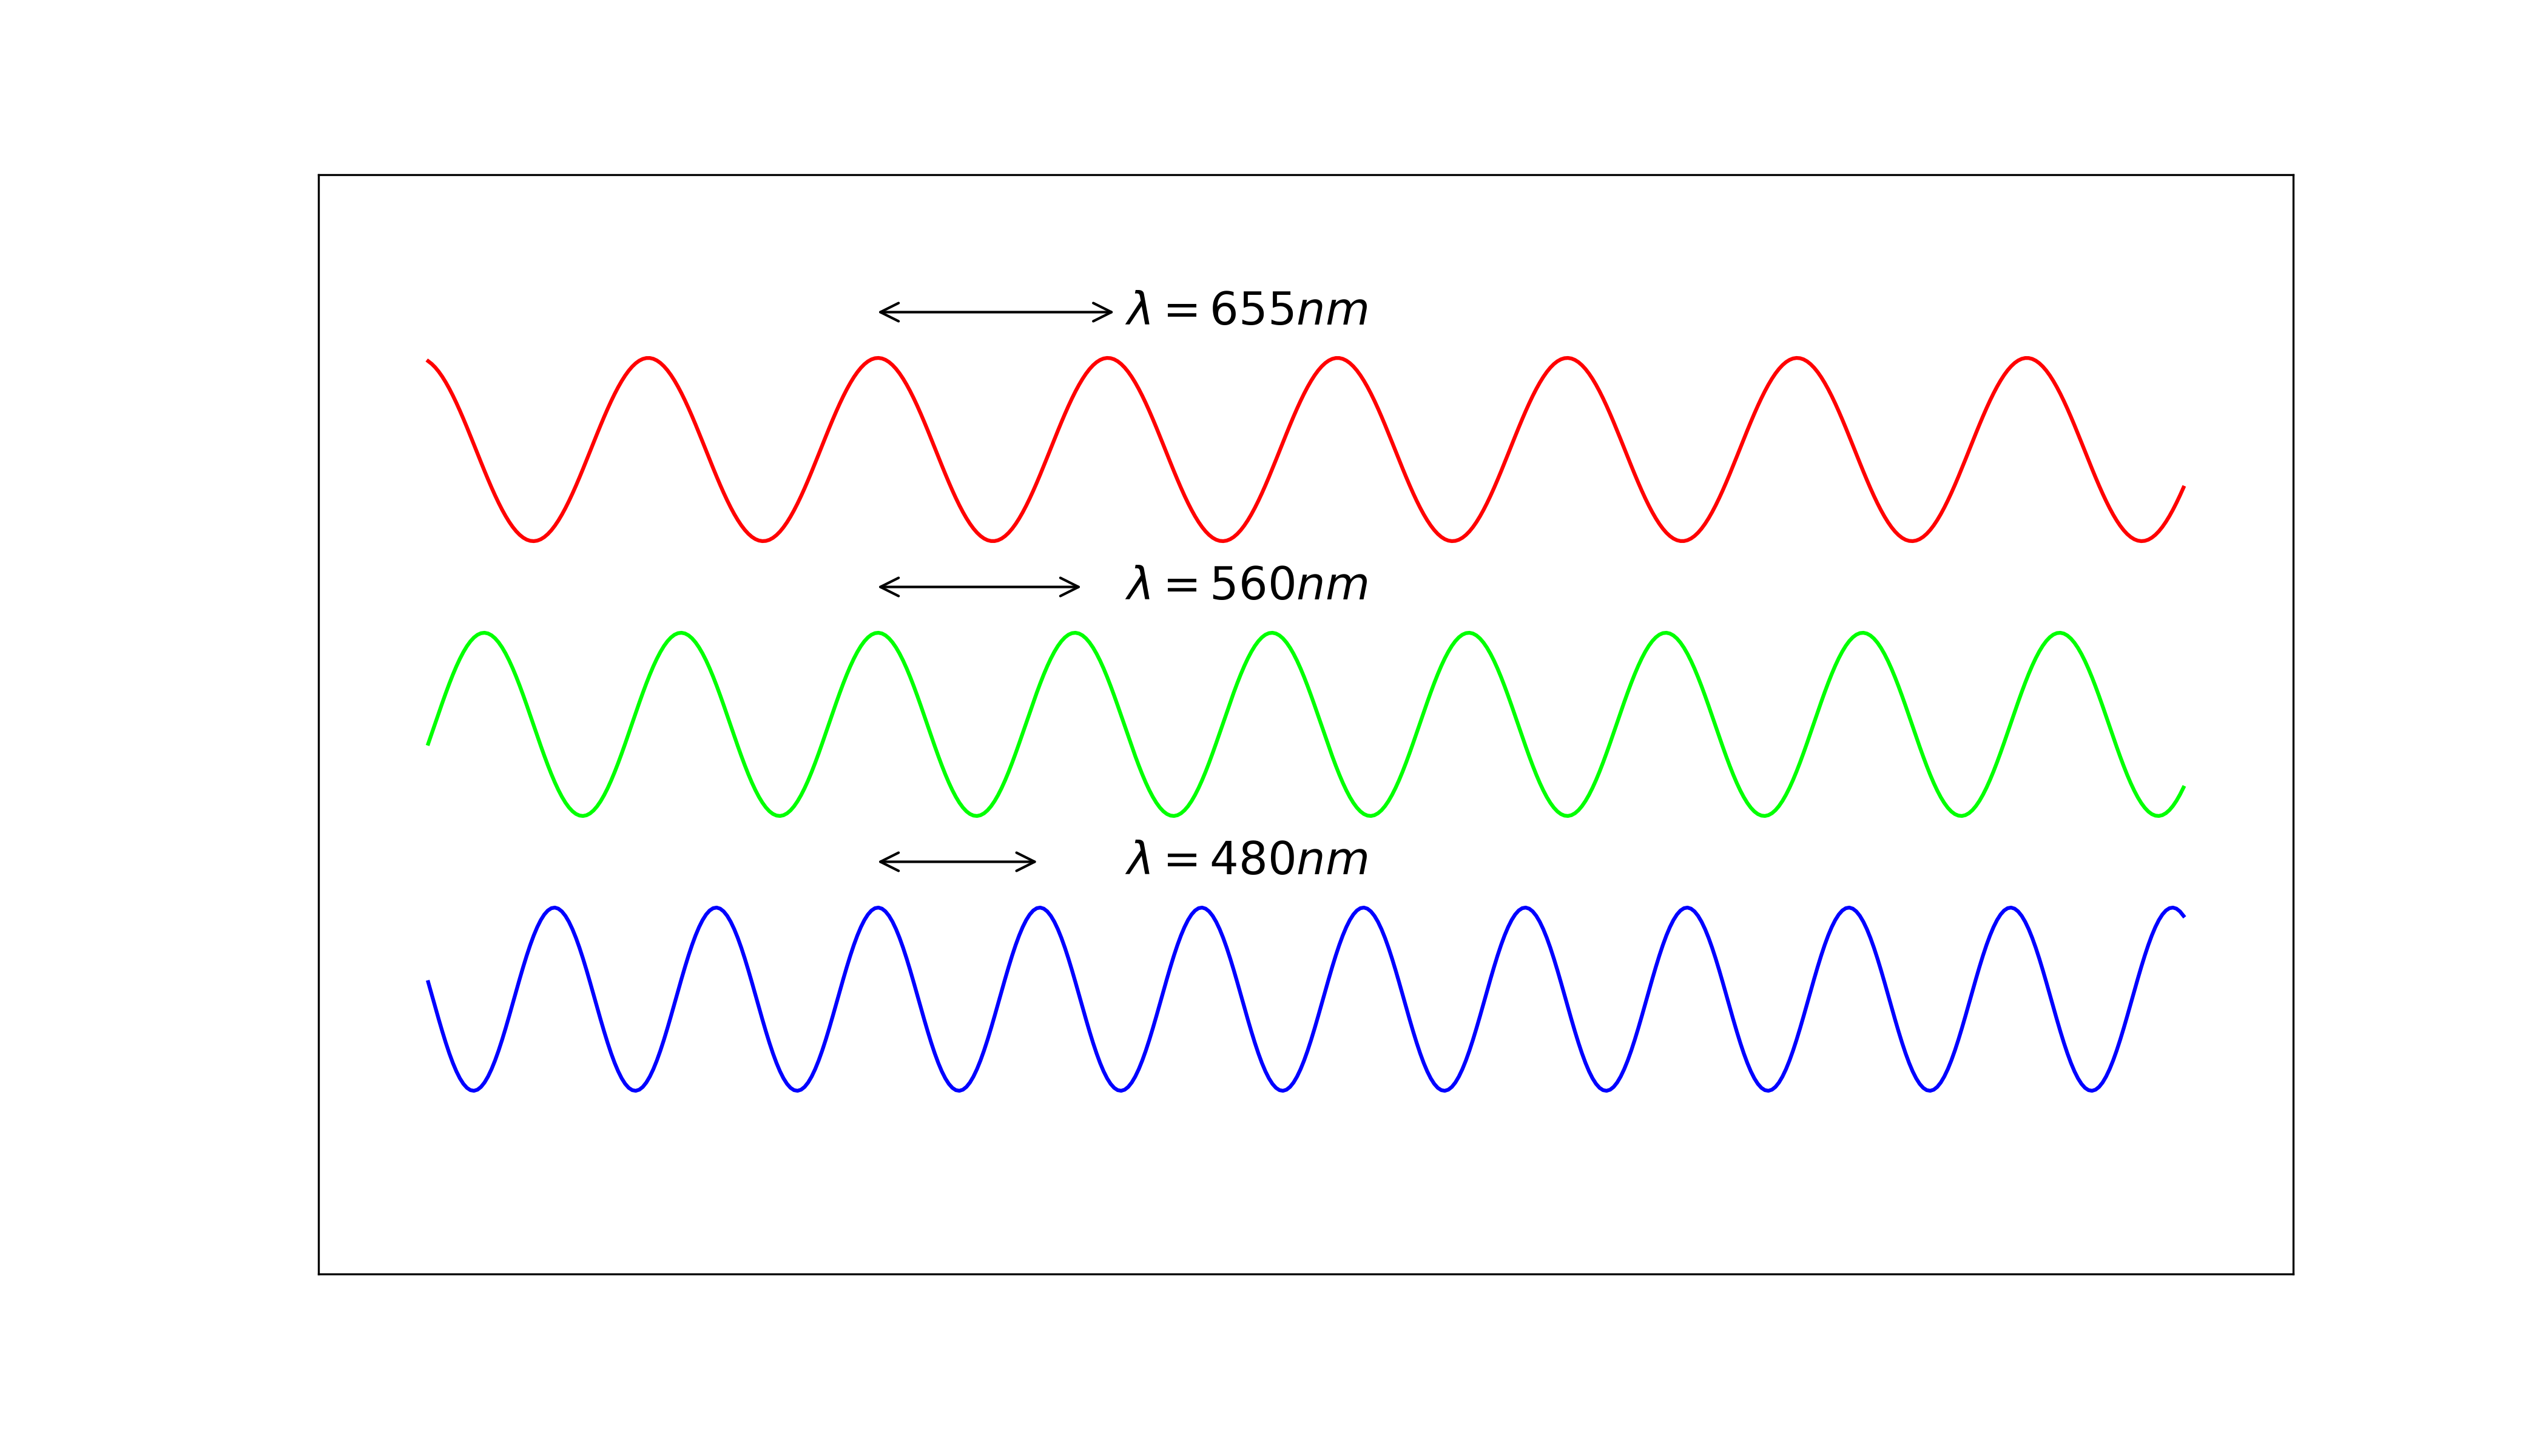
\includegraphics[width=0.8\textwidth]{fig:wave.png}
    \caption{Radiación electromagnética. Cambio de color con la longitud de onda.}
    \label{}
  \end{figure}
\end{frame}
%--- Next Frame ---%

\begin{frame}{\secname : \subsecname}
  \begin{figure}
    \centering
    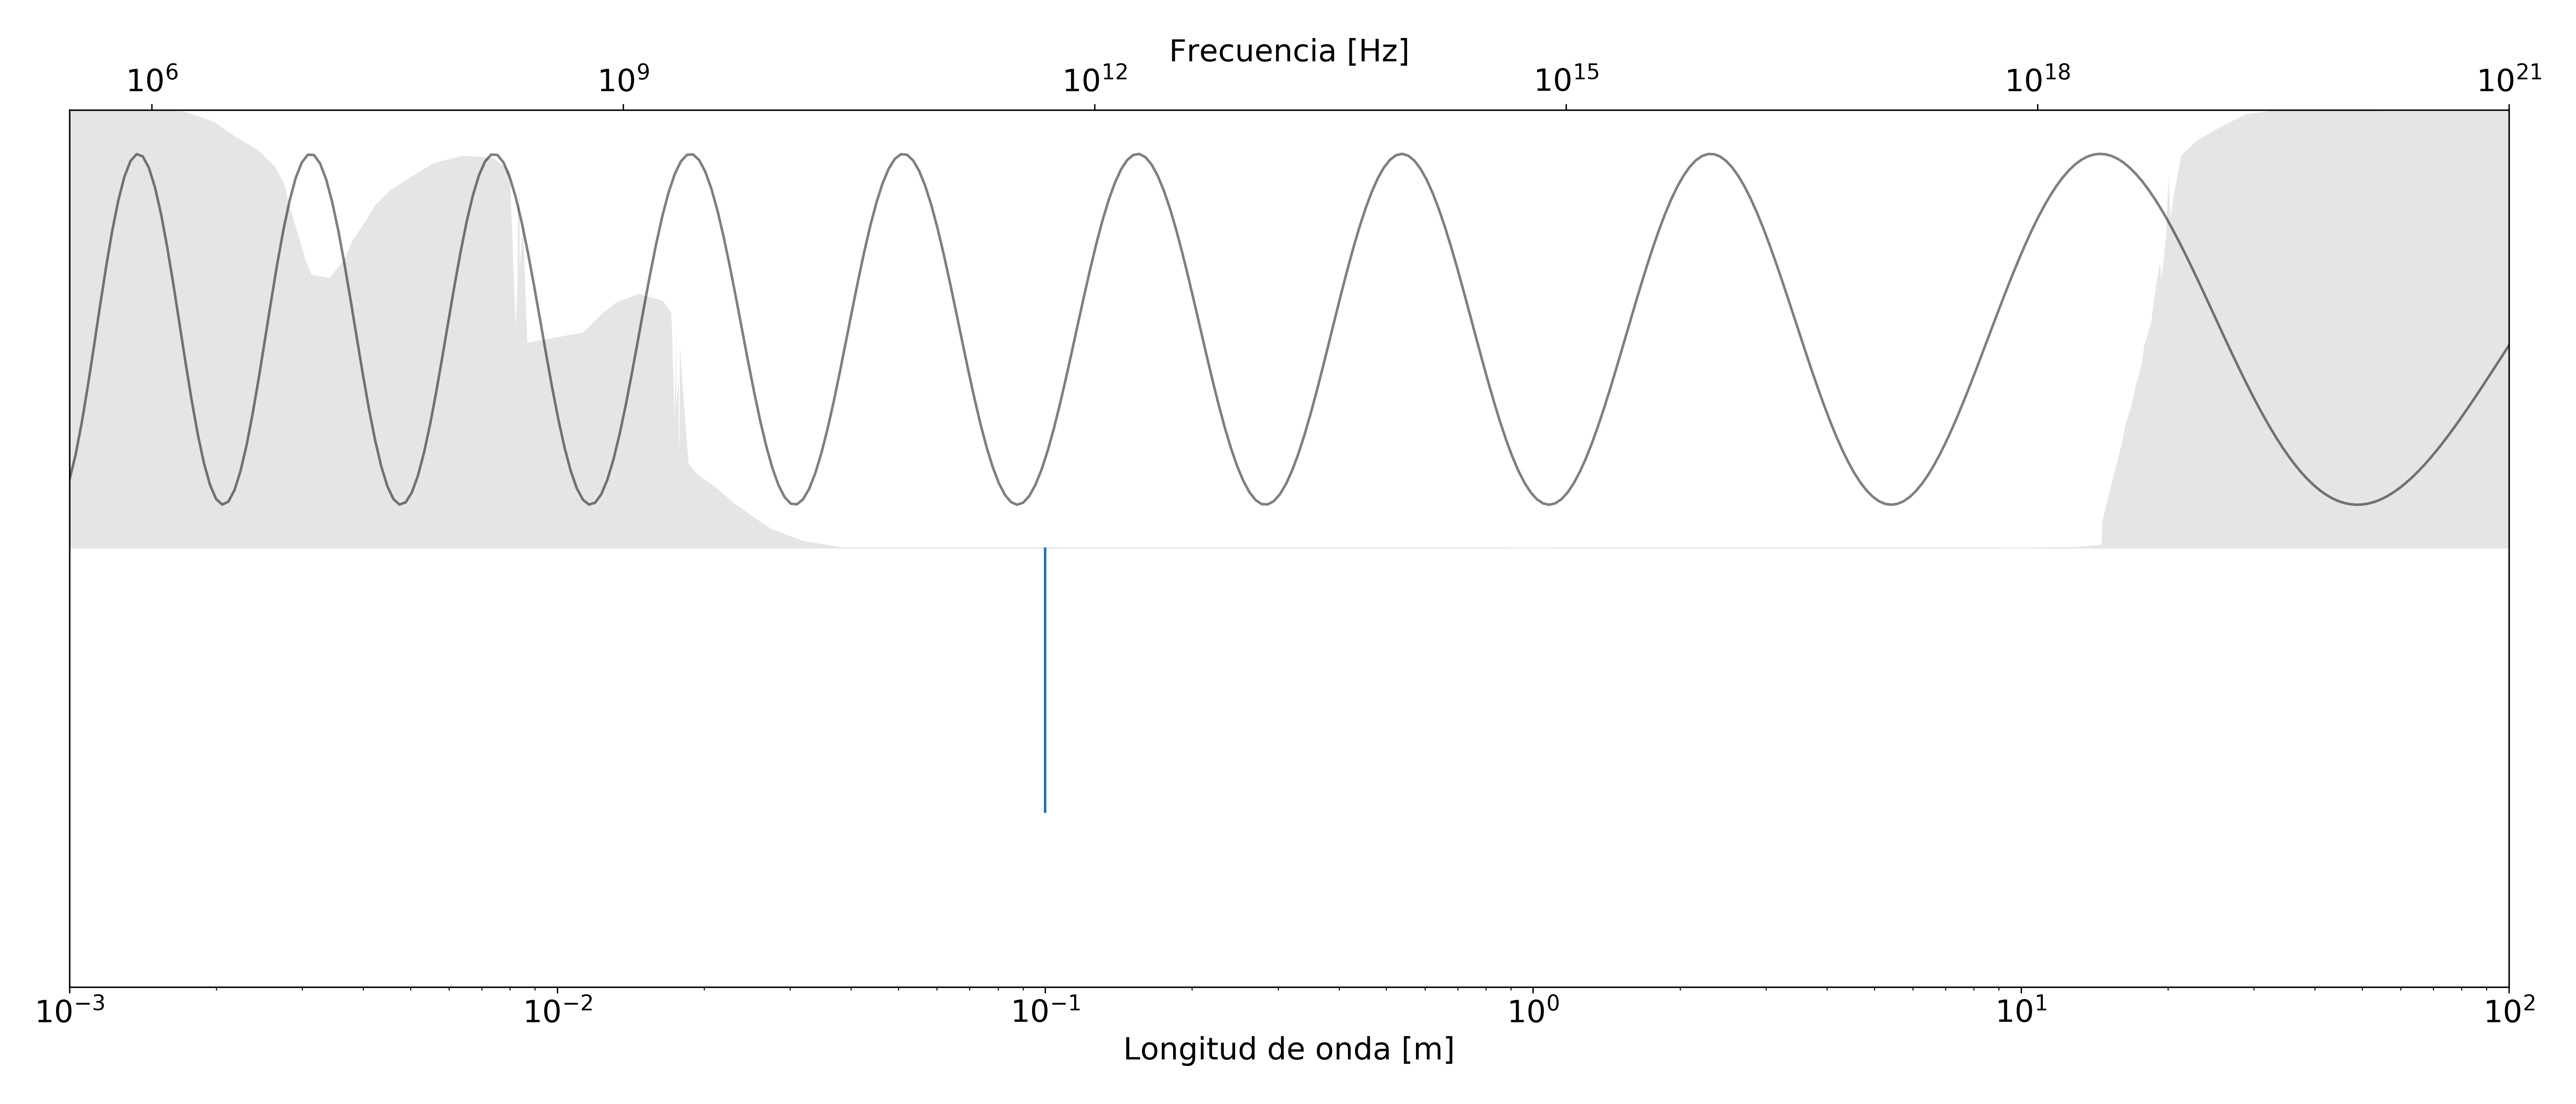
\includegraphics[width=\textwidth]{fig:espectro.png}
    \caption{Espectro electromagnético en longitud de onda (abajo) y frecuencia (arriba).}
    \label{}
  \end{figure}
\end{frame}
%--- Next Frame ---%


\begin{frame}
  \frametitle{Conociendo el espectro}
  \begin{exampleblock}{Ejemplo:}
    \begin{itemize}
      \item Visible
      \begin{itemize}
        \item<1> $[\lambda=450-495 nm]$ {\color{blue} azul}
        \item<1> $[\lambda=495-570 nm]$ {\color{green} verde}
        \item<1> $[\lambda=620-750 nm]$ {\color{red} rojo}
      \end{itemize}
      \item Infrarrojo
      \begin{itemize}
        \item<2> $[\lambda=0.75-1.4\mu m]$ Cercano
        \item<2> $[\lambda=1.4-3\mu m]$ Onda corta
        \item<2> $[\lambda=8-15\mu m]$ Termico
      \end{itemize}
      \item Microondas - SAR
      \begin{itemize}
        \item<3> $[\nu = 26.5 -18.0 GHz]$ Banda K
        \item<3> $[\nu = 12.5 - 8.0 GHz]$ Banda X
        \item<3> $[\nu = 2.0 - 1.0 GHz] $ Banda L
      \end{itemize}
    \end{itemize}
  \end{exampleblock}
\end{frame}

%--- Next Frame ---%

\begin{frame}{\secname : \subsecname}
  \begin{figure}
    \centering
    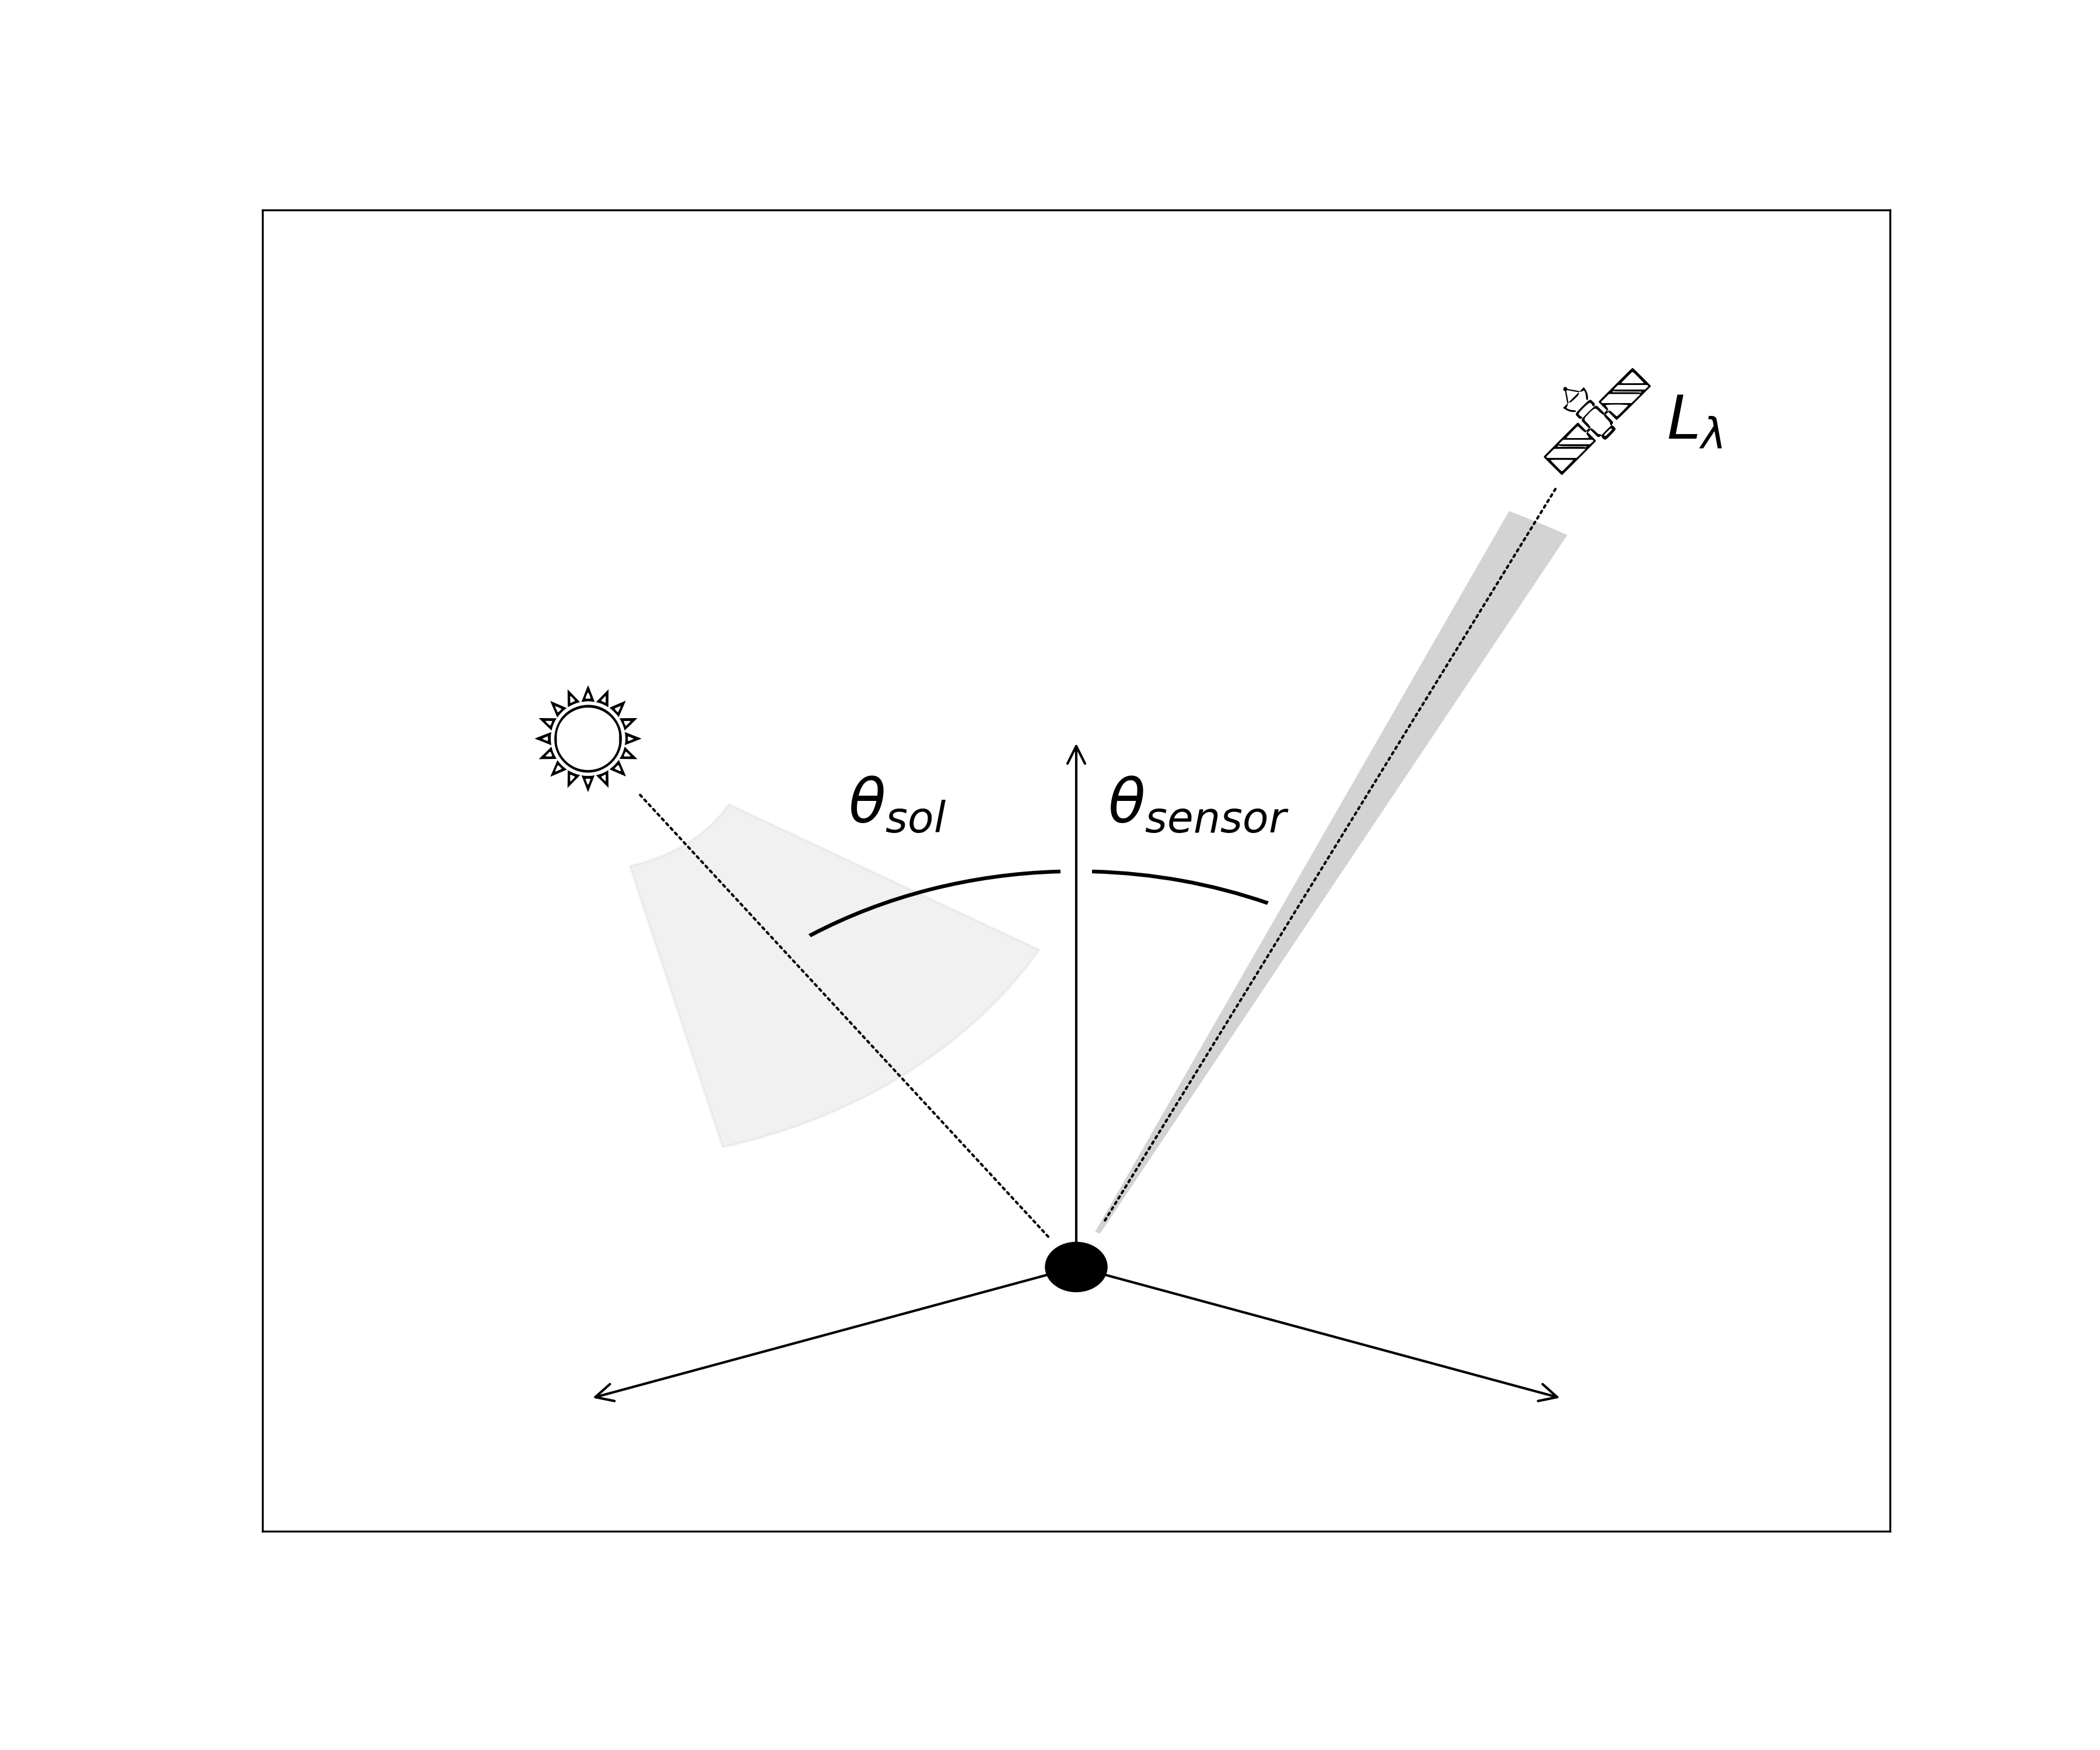
\includegraphics[width=0.57\textwidth]{fig:geometria.png}
    \caption{Radiancia como unidad en teledetección.}
    \label{}
  \end{figure}
\end{frame}
%--- Next Frame ---%

\begin{frame}{\secname : \subsecname}
  \begin{figure}
    \centering
    \movie[width = 0.8\textwidth,loop,autostart]{\centering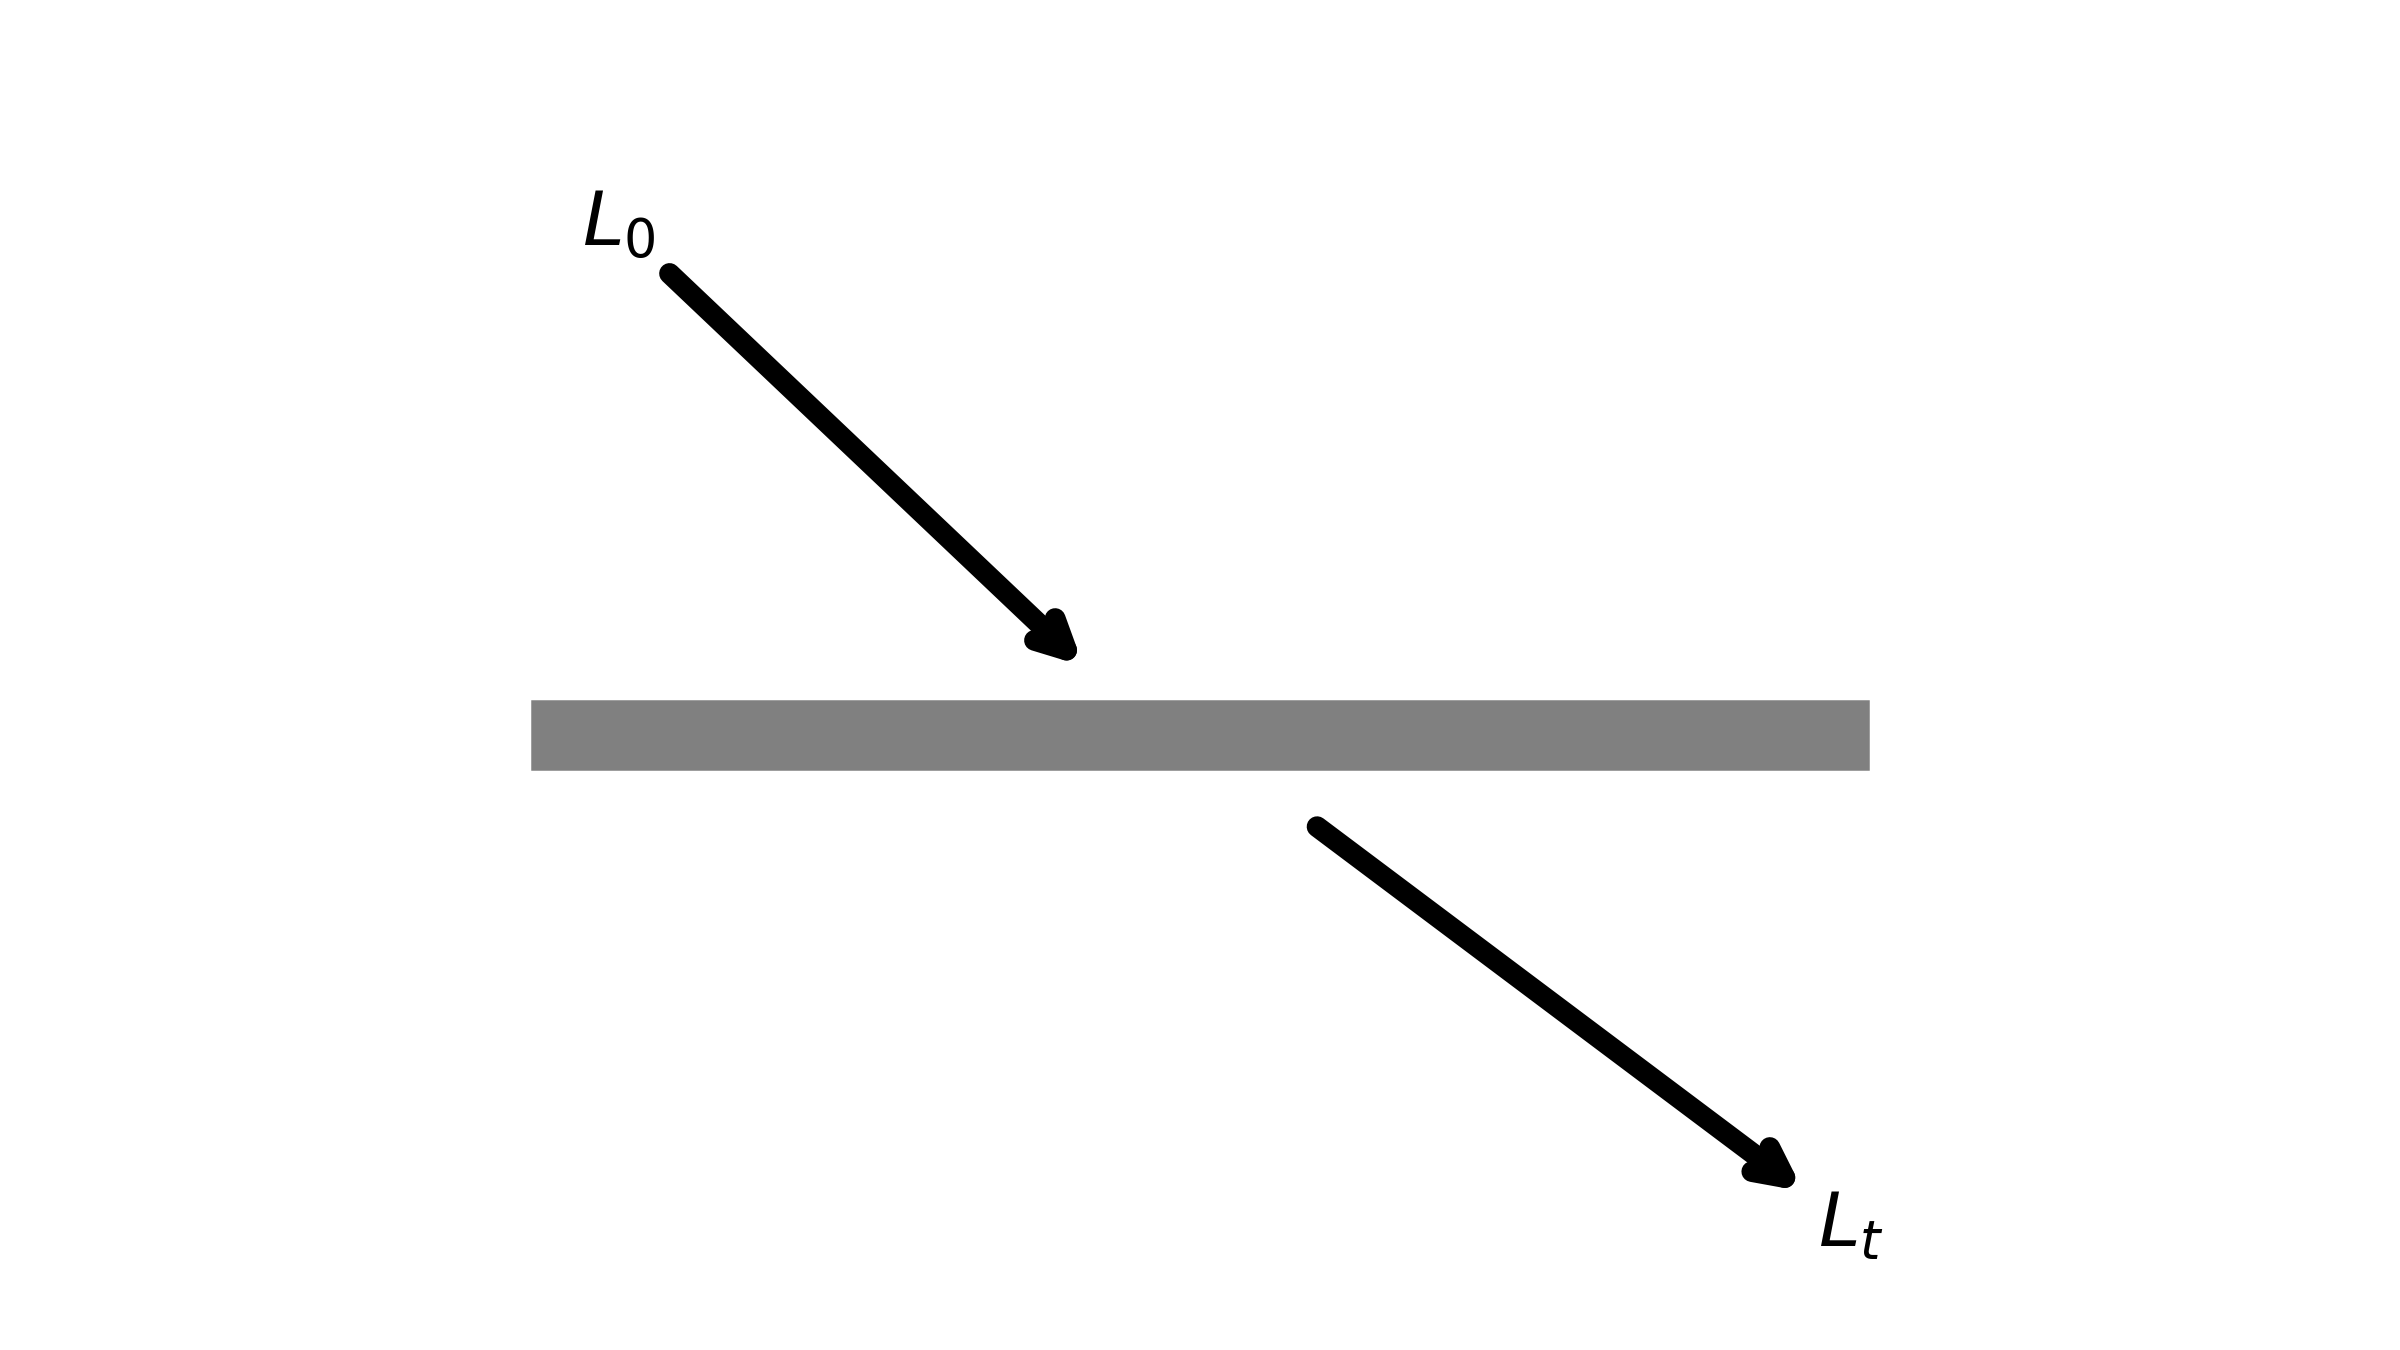
\includegraphics[width=0.8\textwidth]{fig:transmision.png}}{./figs/fig:transmision.mp4}
    \caption{Interacción entre materia y radiación: transmitancia.}
    \label{}
  \end{figure}
\end{frame}
%--- Next Frame ---%

\begin{frame}{\secname : \subsecname}
  \begin{figure}
    \centering
    \movie[width = 0.8\textwidth,loop,autostart]{\centering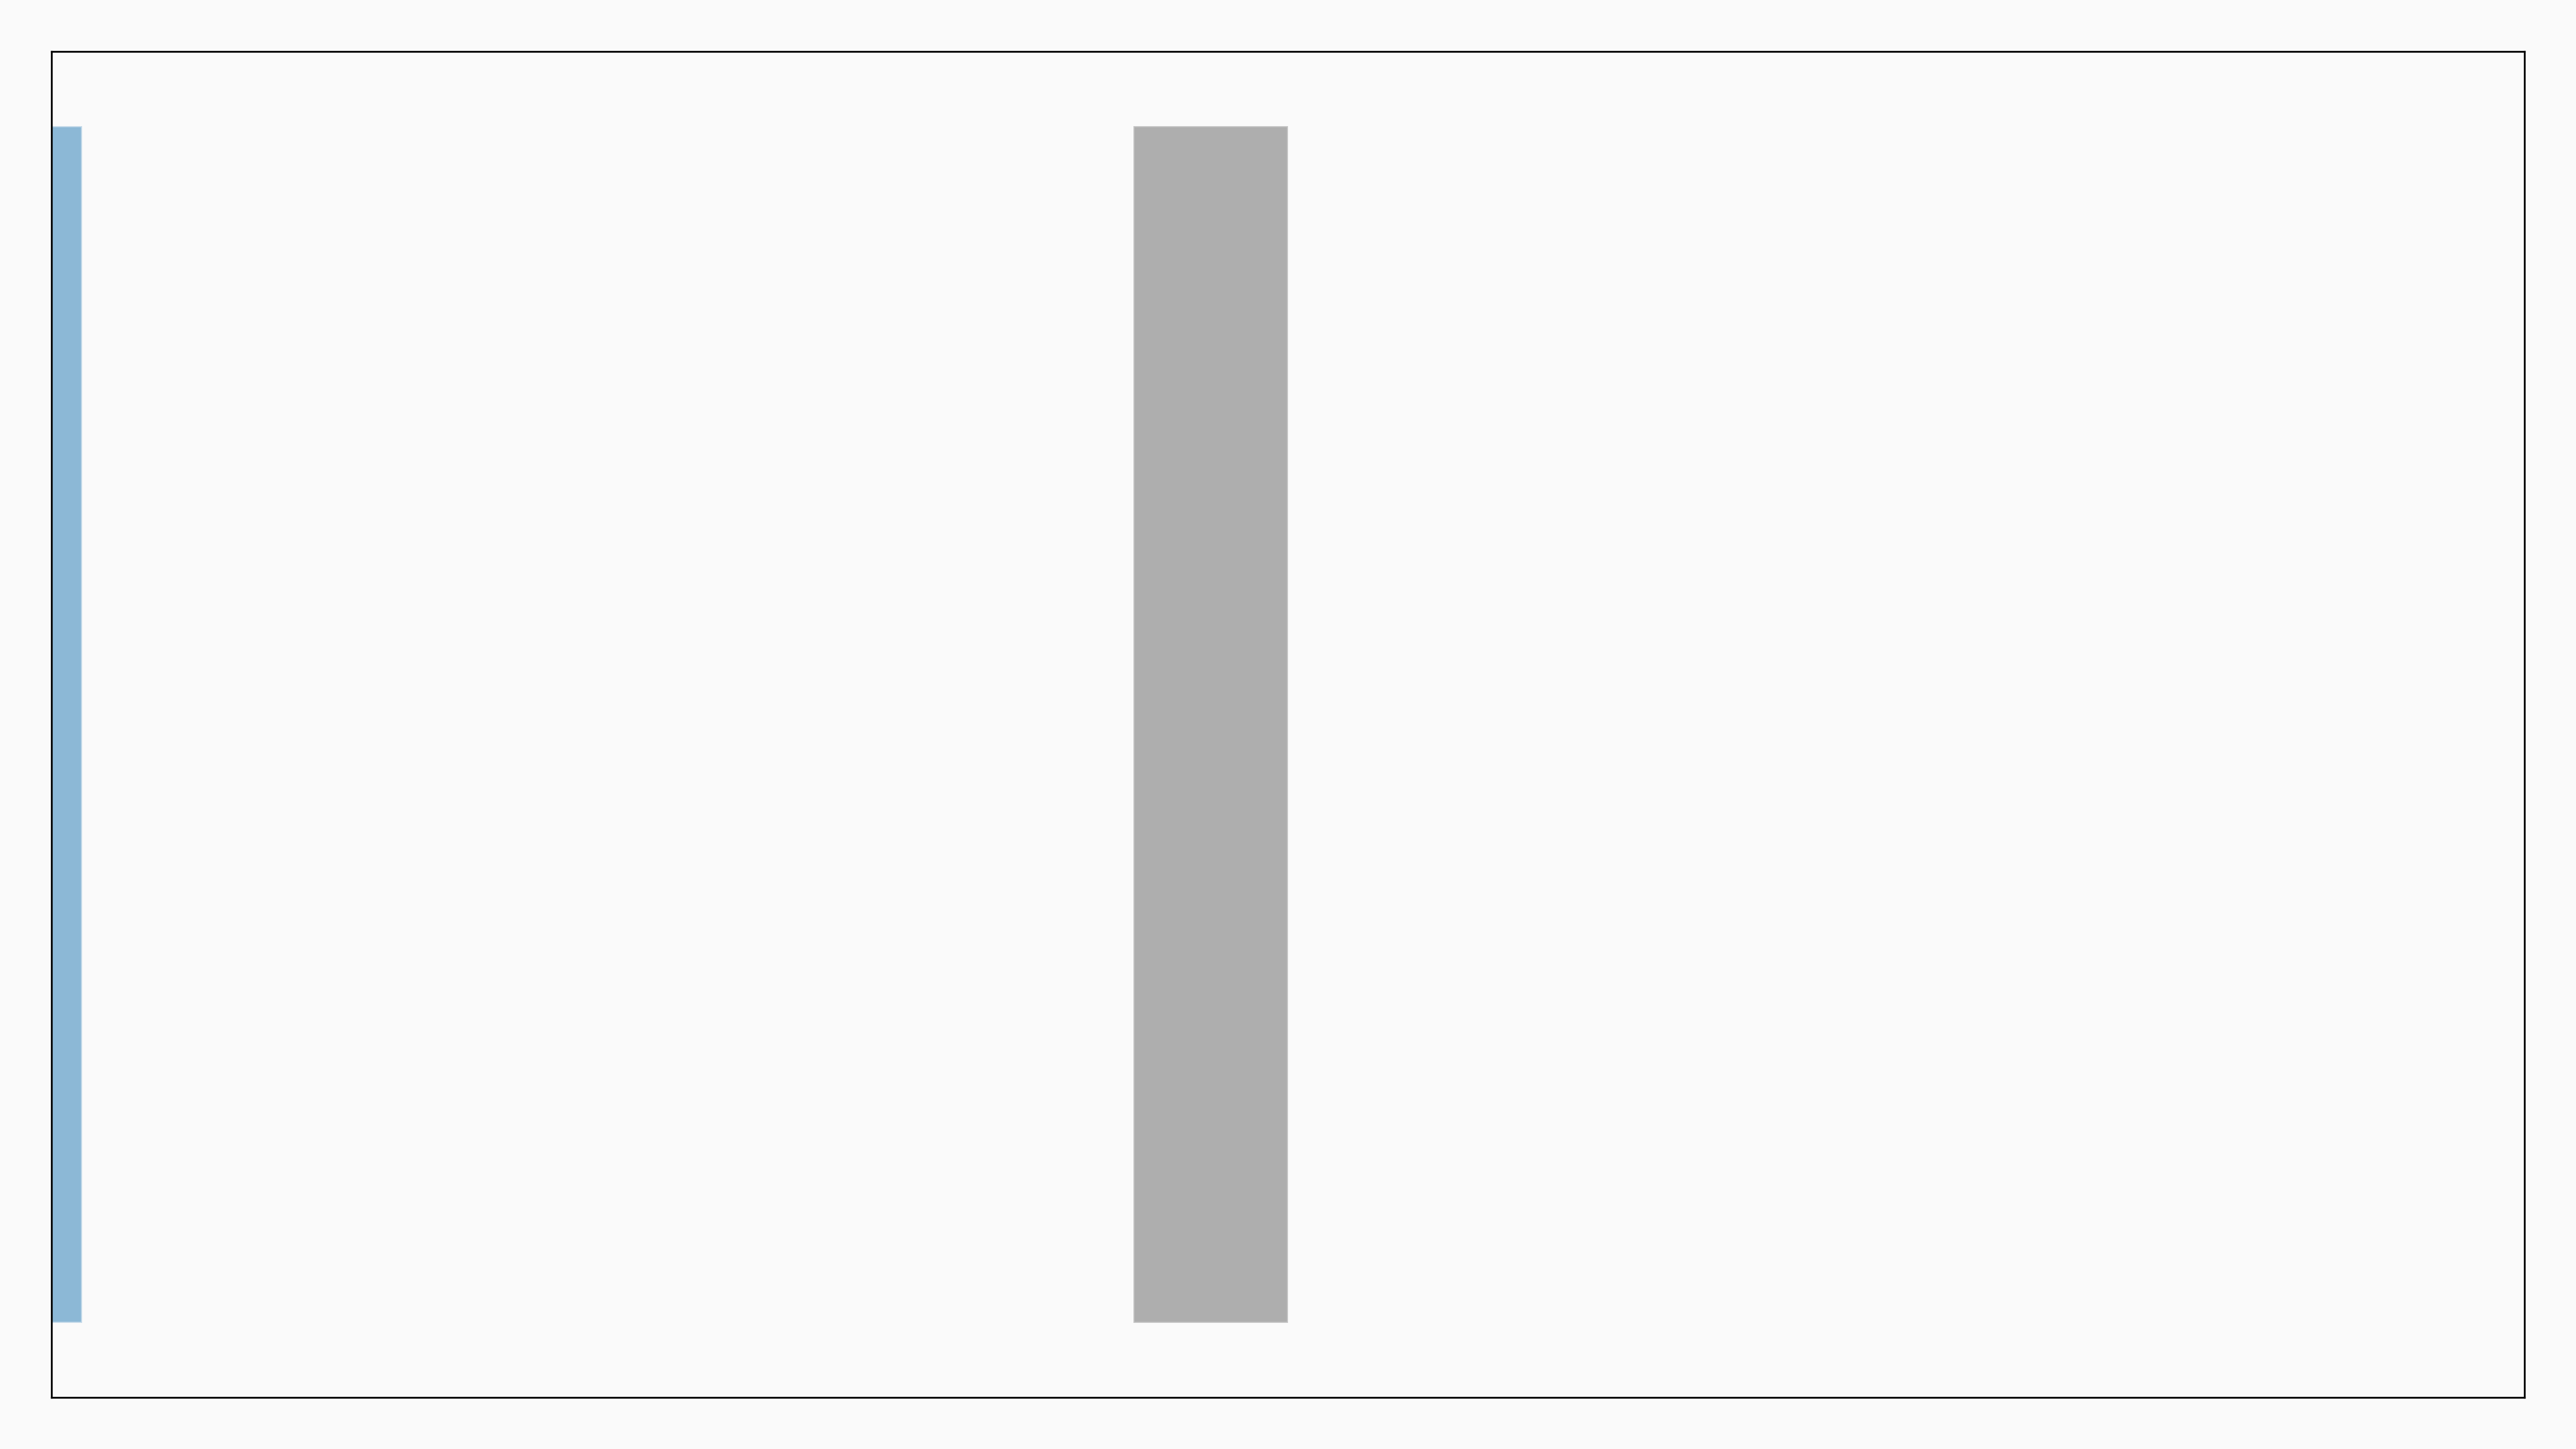
\includegraphics[width=0.8\textwidth]{fig:absorcion.png}}{./figs/fig:absorcion.mp4}
    \caption{Interacción entre materia y radiación: absorvancia.}
    \label{}
  \end{figure}
\end{frame}
%--- Next Frame ---%

\begin{frame}{\secname : \subsecname}
  \begin{figure}
    \centering
    \movie[width = 0.8\textwidth,loop,autostart]{\centering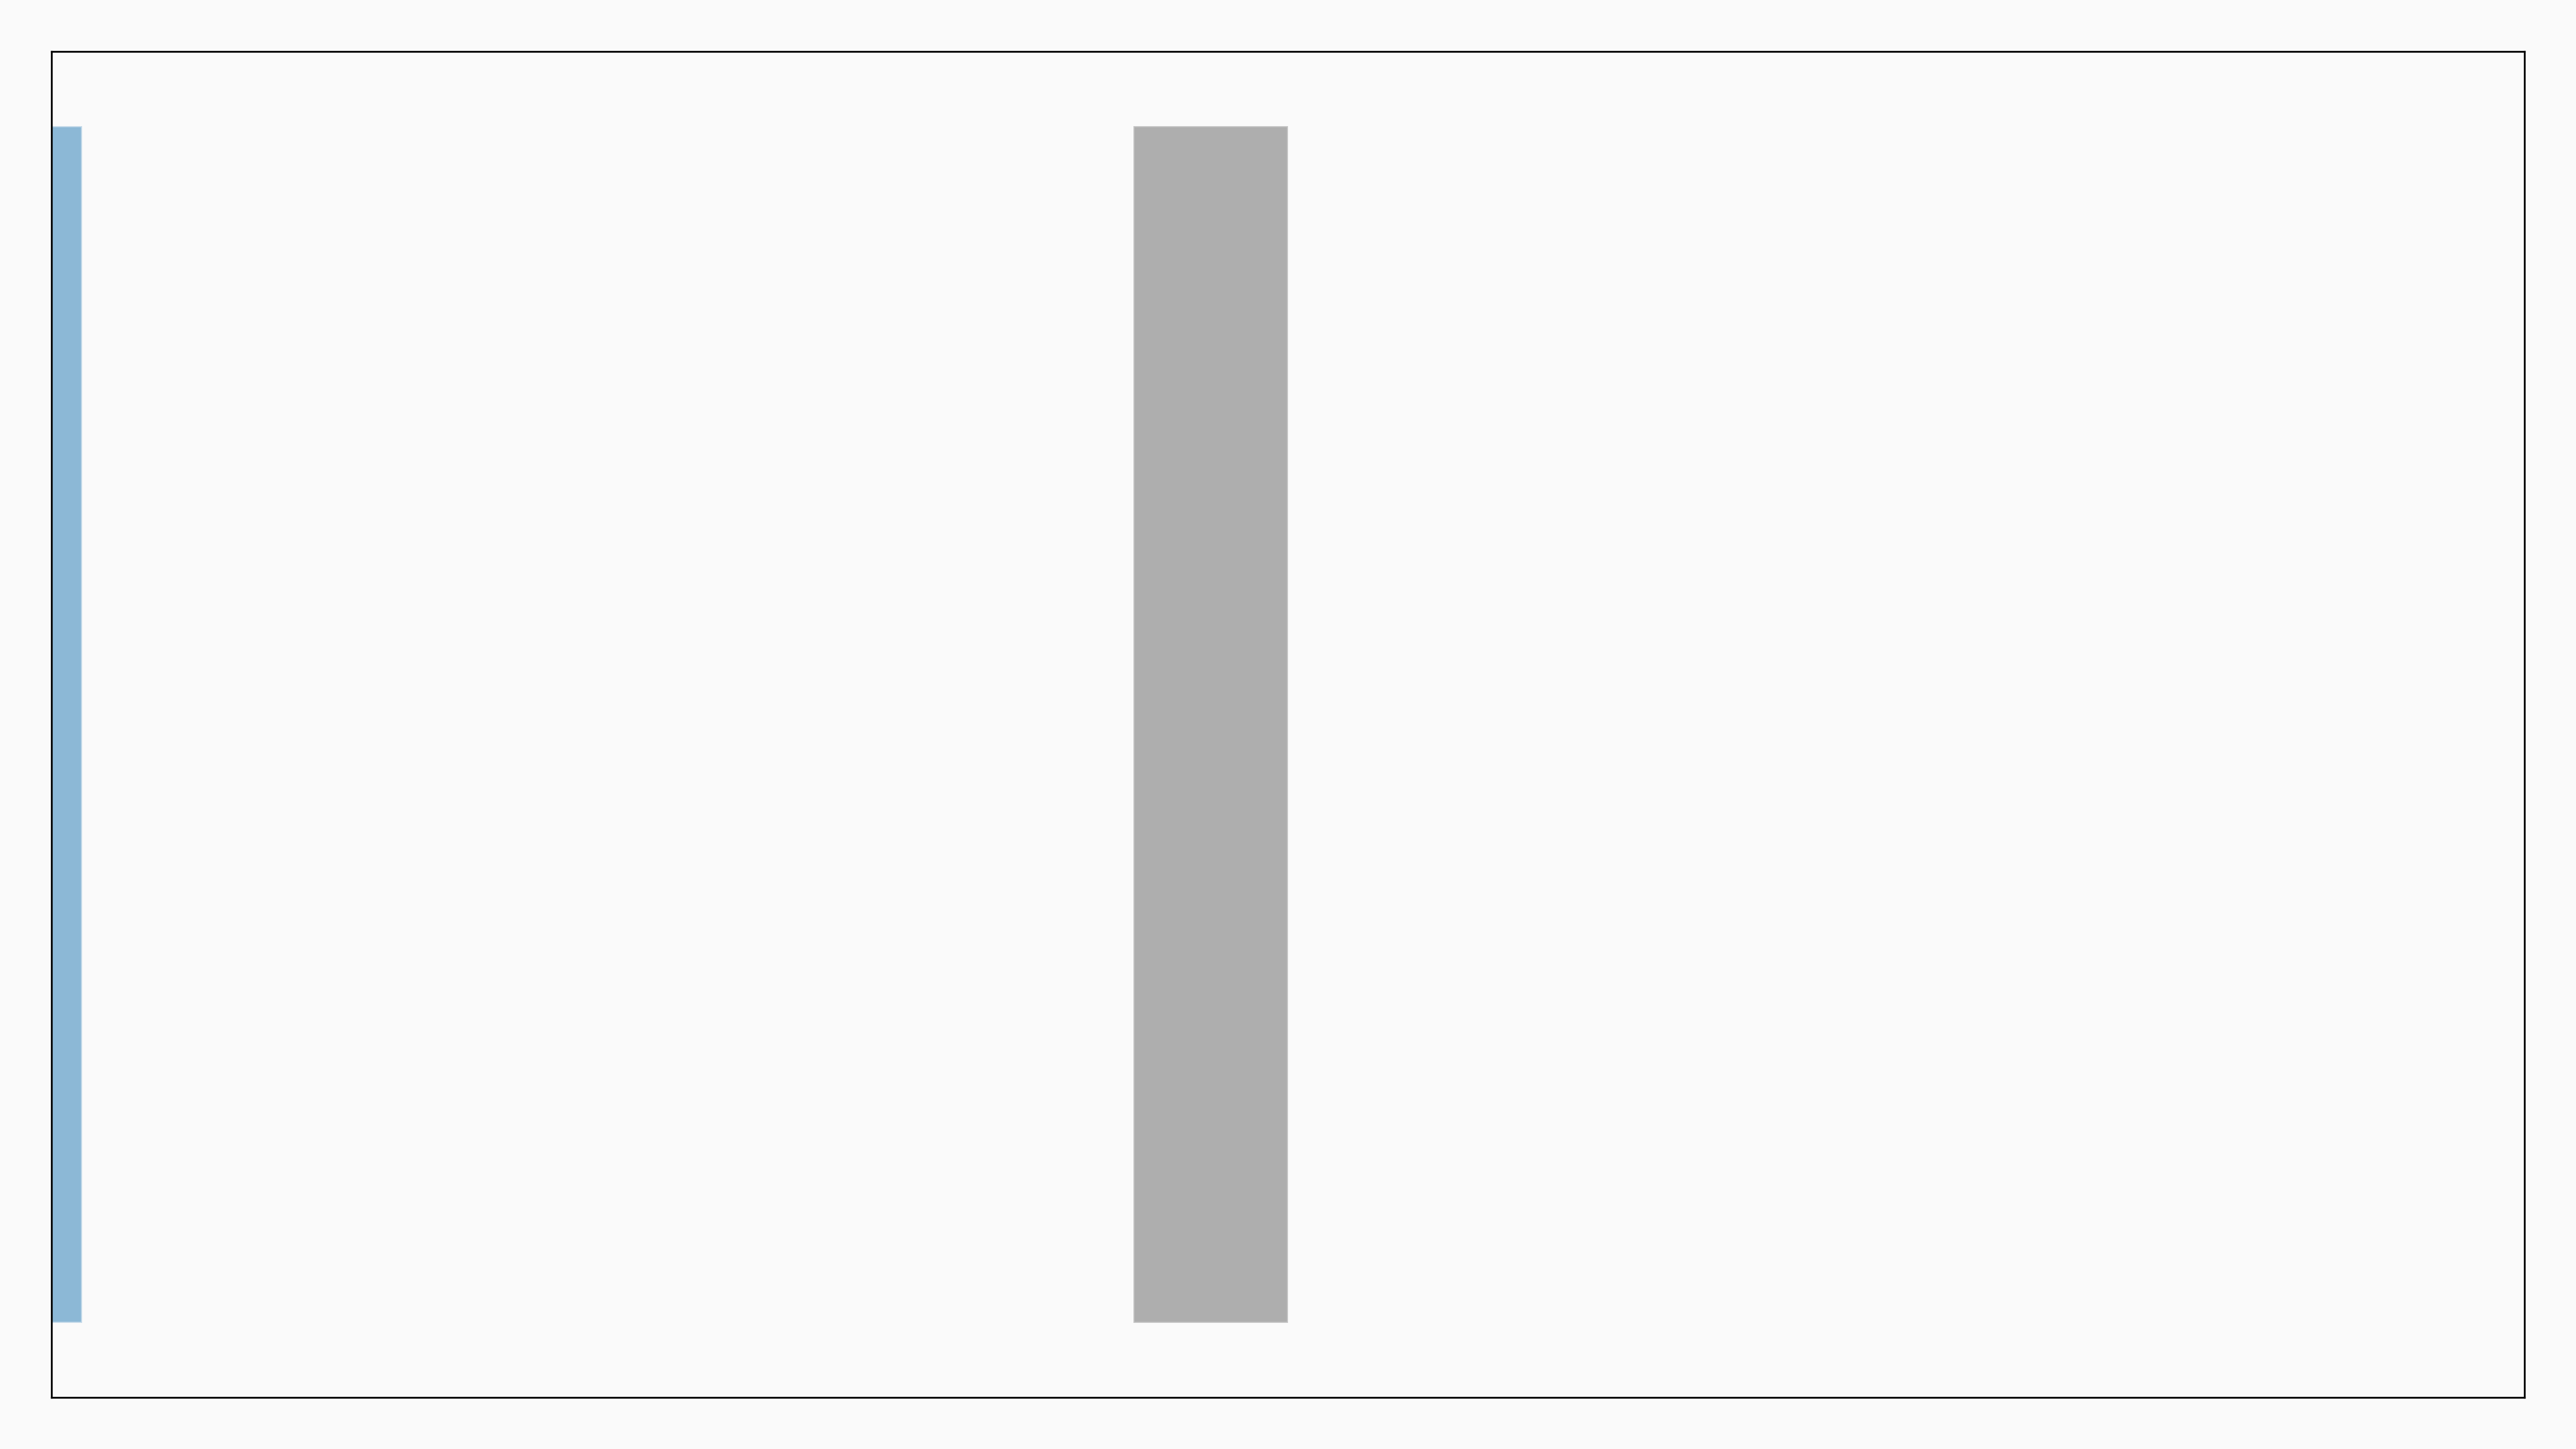
\includegraphics[width=0.8\textwidth]{fig:refleccion.png}}{./figs/fig:refleccion.mp4}
    \caption{Interacción entre materia y radiación: reflectancia.}
    \label{}
  \end{figure}
\end{frame}
%--- Next Frame ---%

\begin{frame}{\secname : \subsecname}
    \begin{block}{Definición}
        En función de las radiancas podemos definir la absorvancia, la transmitancia y la reflectancia como
        \begin{equation}
          A_\lambda = \frac{L_{a,\lambda}}{L_{0,\lambda}} ,
        \end{equation}
        \begin{equation}
          T_\lambda = \frac{L_{t,\lambda}}{L_{0,\lambda}} ,
        \end{equation}
        \begin{equation}
          R_\lambda = \frac{L_{r,\lambda}}{L_{0,\lambda}}
        \end{equation}
    \end{block}
\end{frame}
%--- Next Frame ---%

\begin{frame}{\secname : \subsecname}
    \begin{block}{Reflectancia}
        Usaremos la siguiente definición:
        \begin{equation}
          \rho_\lambda = \frac{\pi L_{r,\lambda}}{E_{0,\lambda} \cos \theta_{sol}}
        \end{equation}
    \end{block}
\end{frame}
%--- Next Frame ---%

\subsection{Firmas espectrales}

\begin{frame}{\secname : \subsecname}
  \begin{figure}
    \centering
    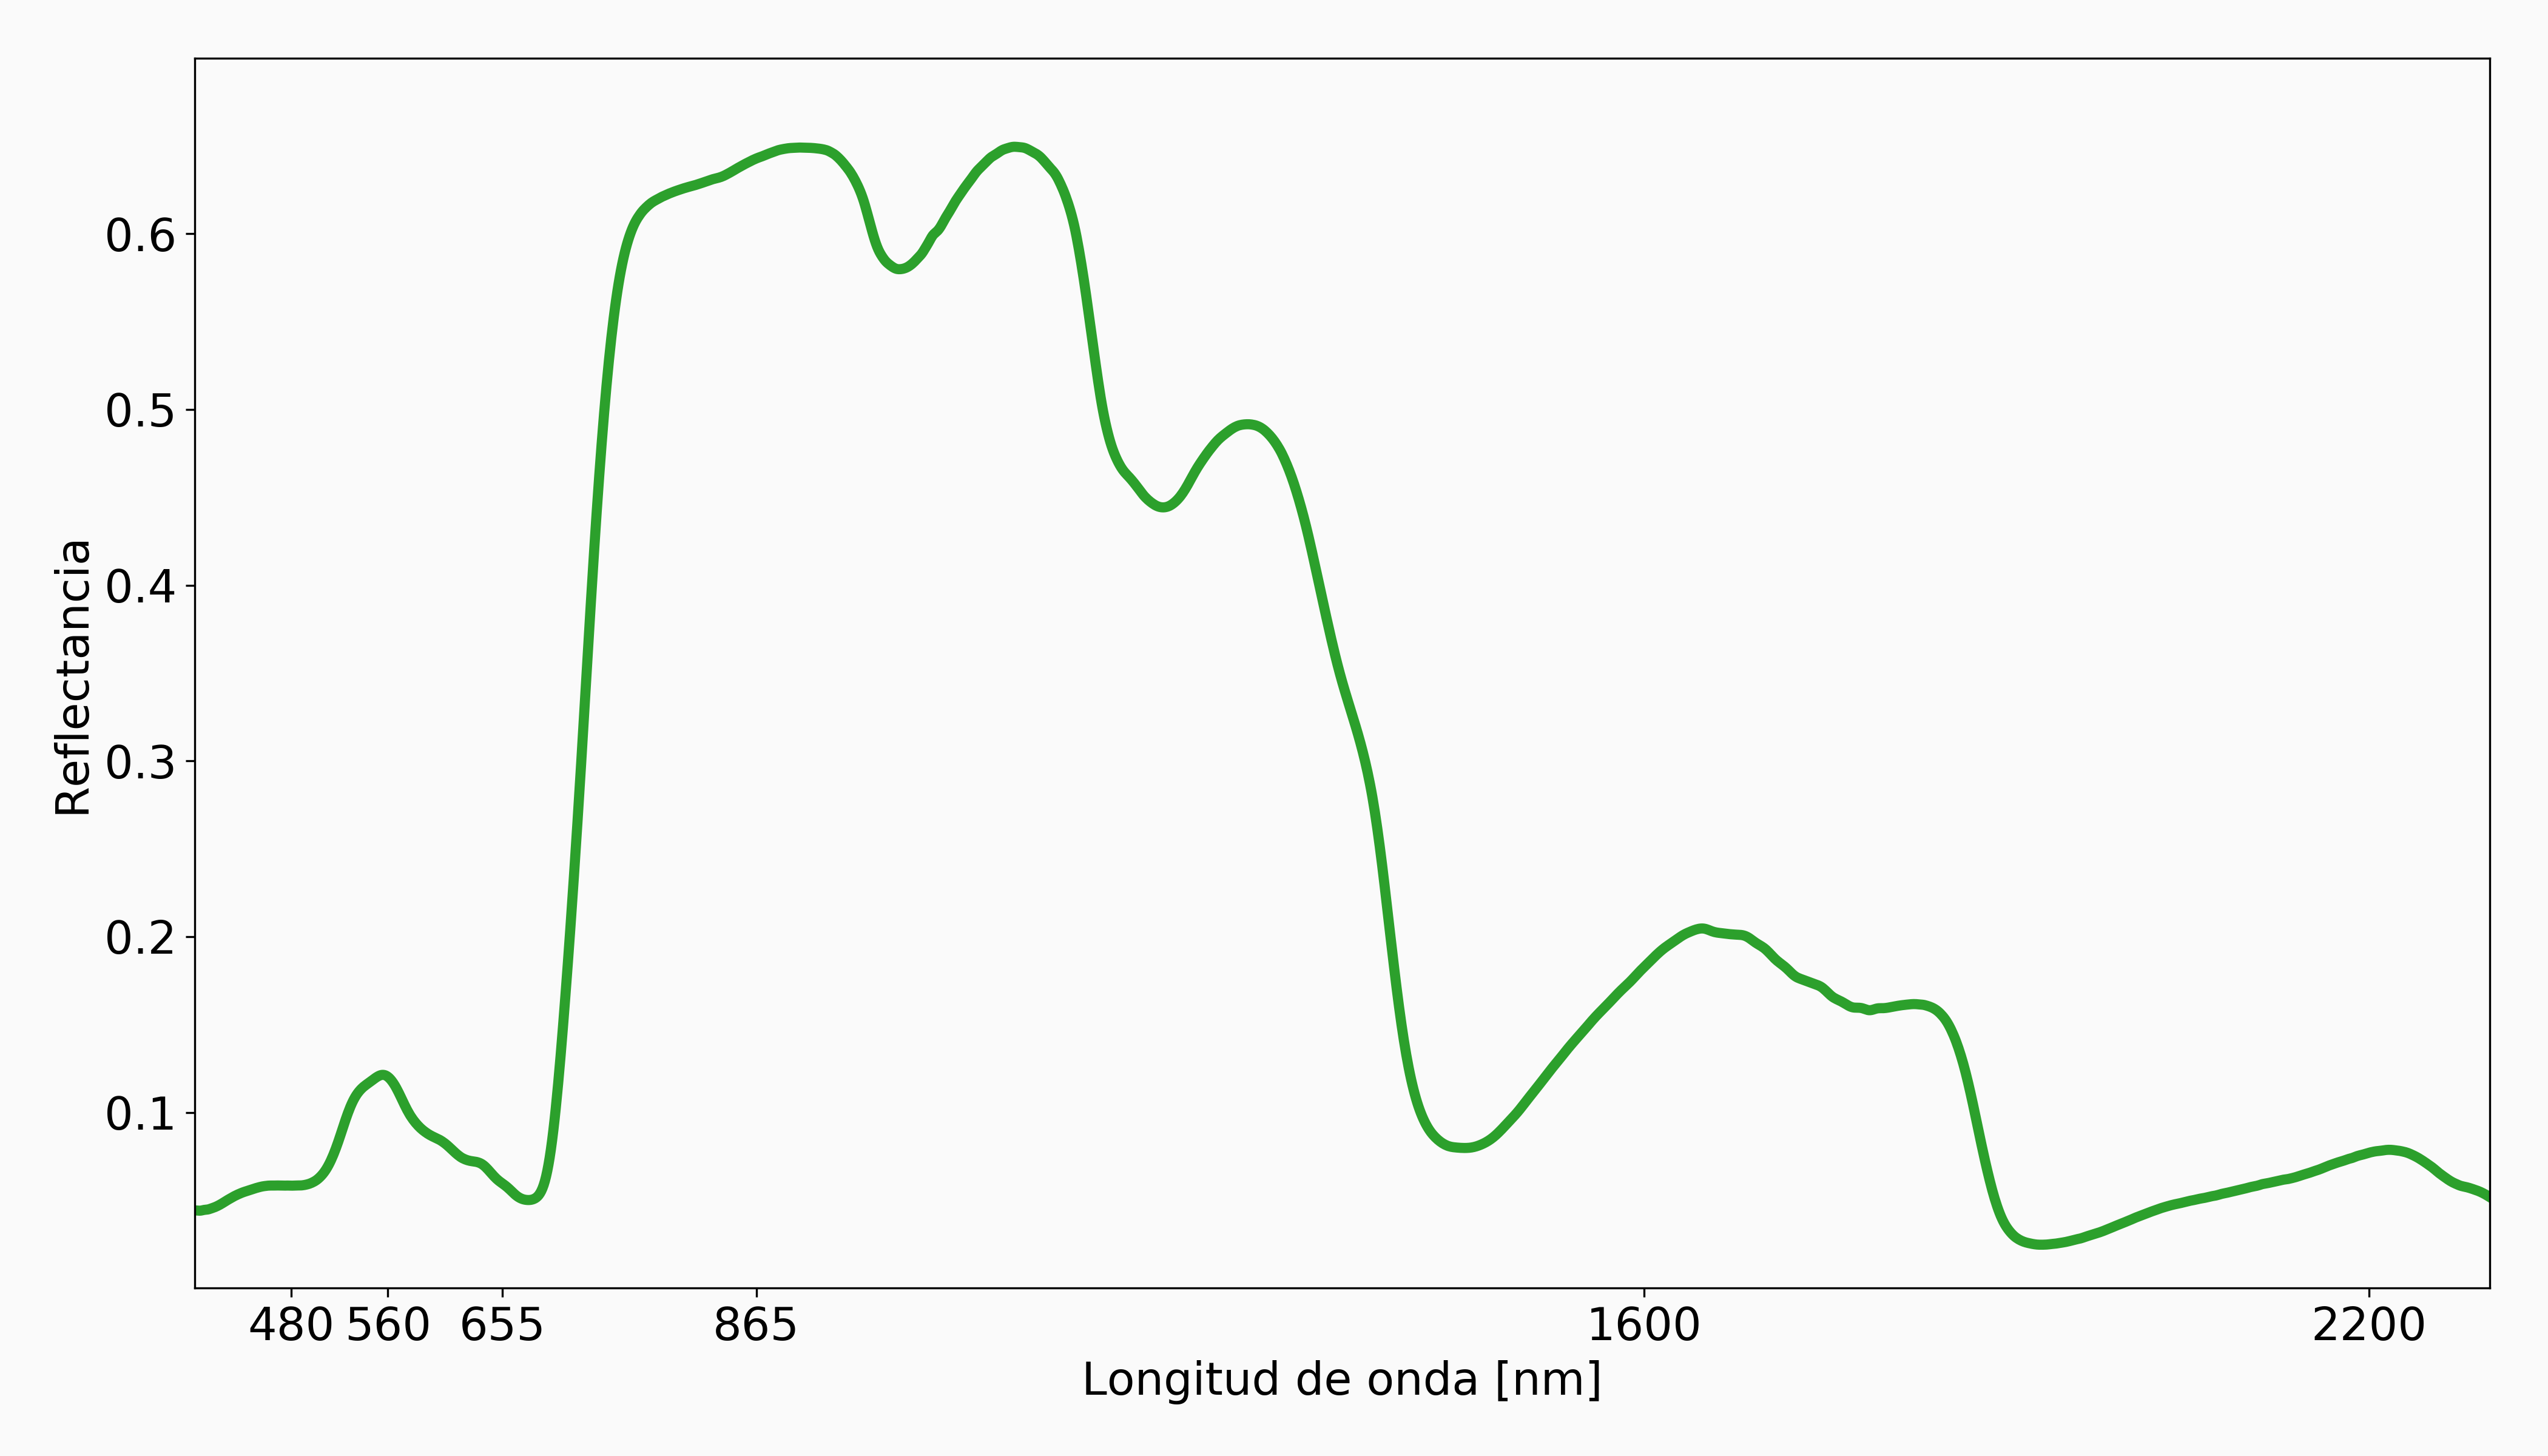
\includegraphics[width=0.8\textwidth]{fig:v.png}
    \caption{Firmas espectral de la vegetación.}
    \label{}
  \end{figure}
\end{frame}
%--- Next Frame ---%

\begin{frame}{\secname : \subsecname}
  \begin{figure}
    \centering
    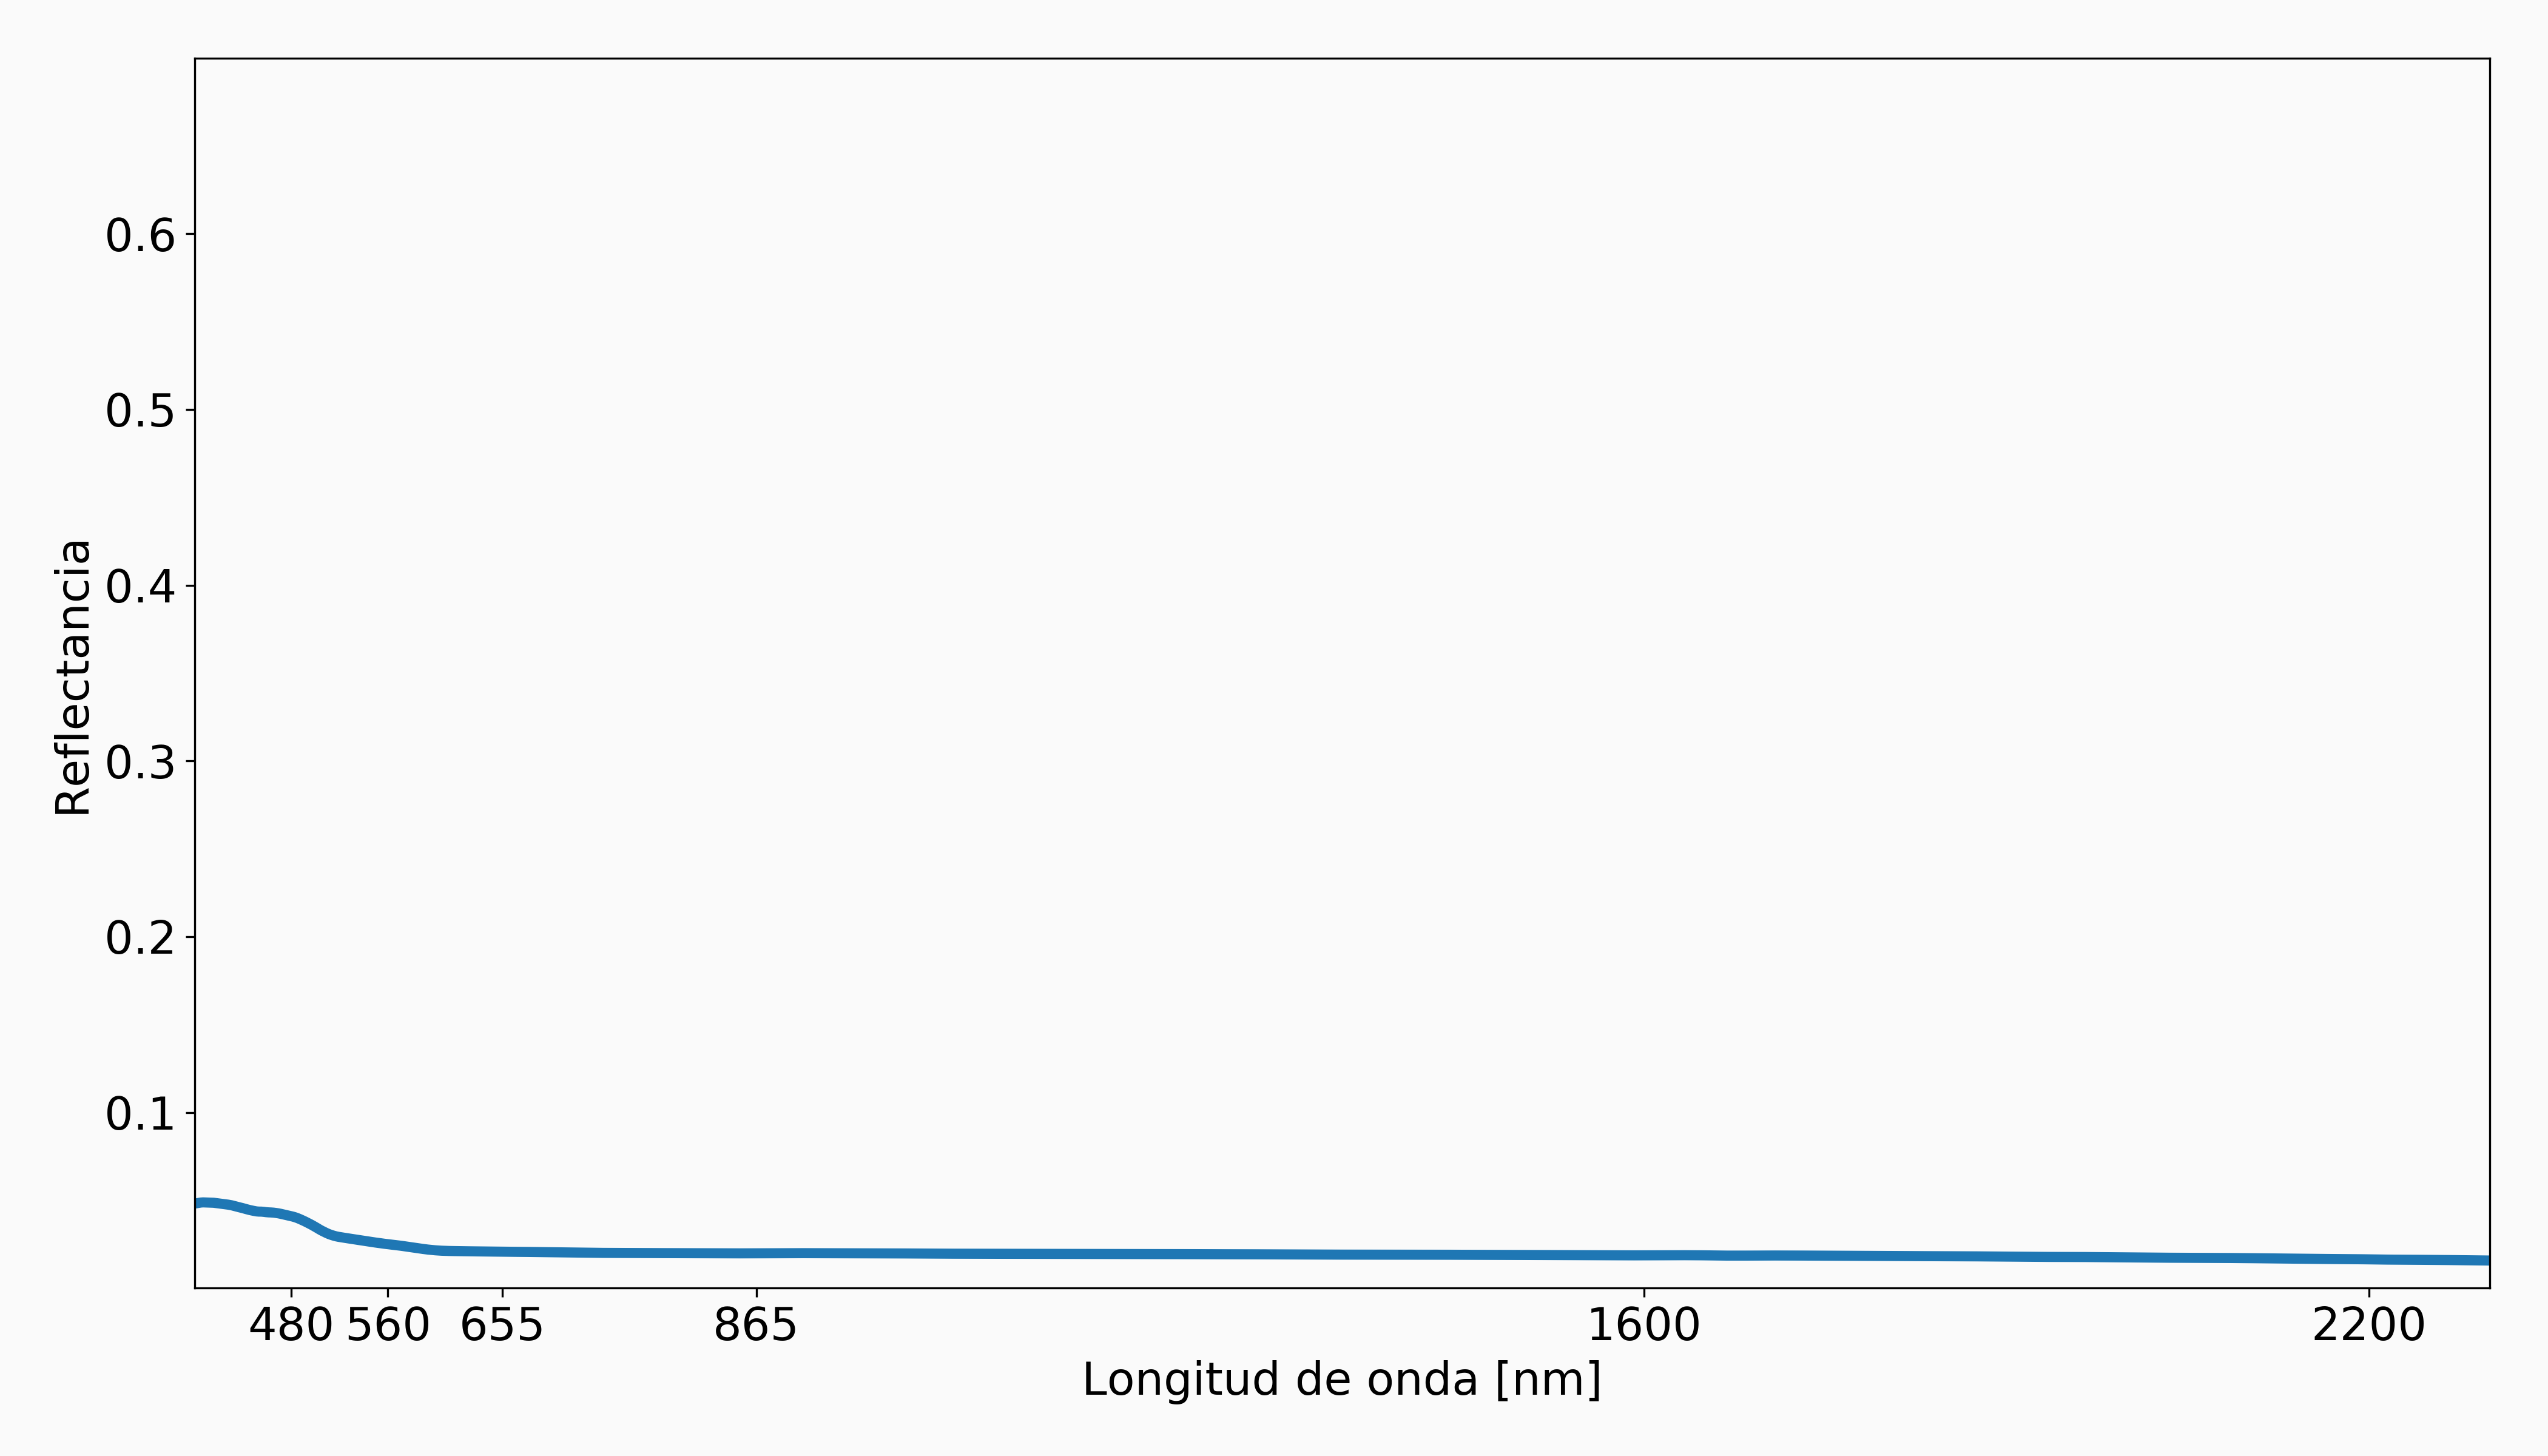
\includegraphics[width=0.8\textwidth]{fig:a.png}
    \caption{Firmas espectral de la agua.}
    \label{}
  \end{figure}
\end{frame}
%--- Next Frame ---%

\begin{frame}{\secname : \subsecname}
  \begin{figure}
    \centering
    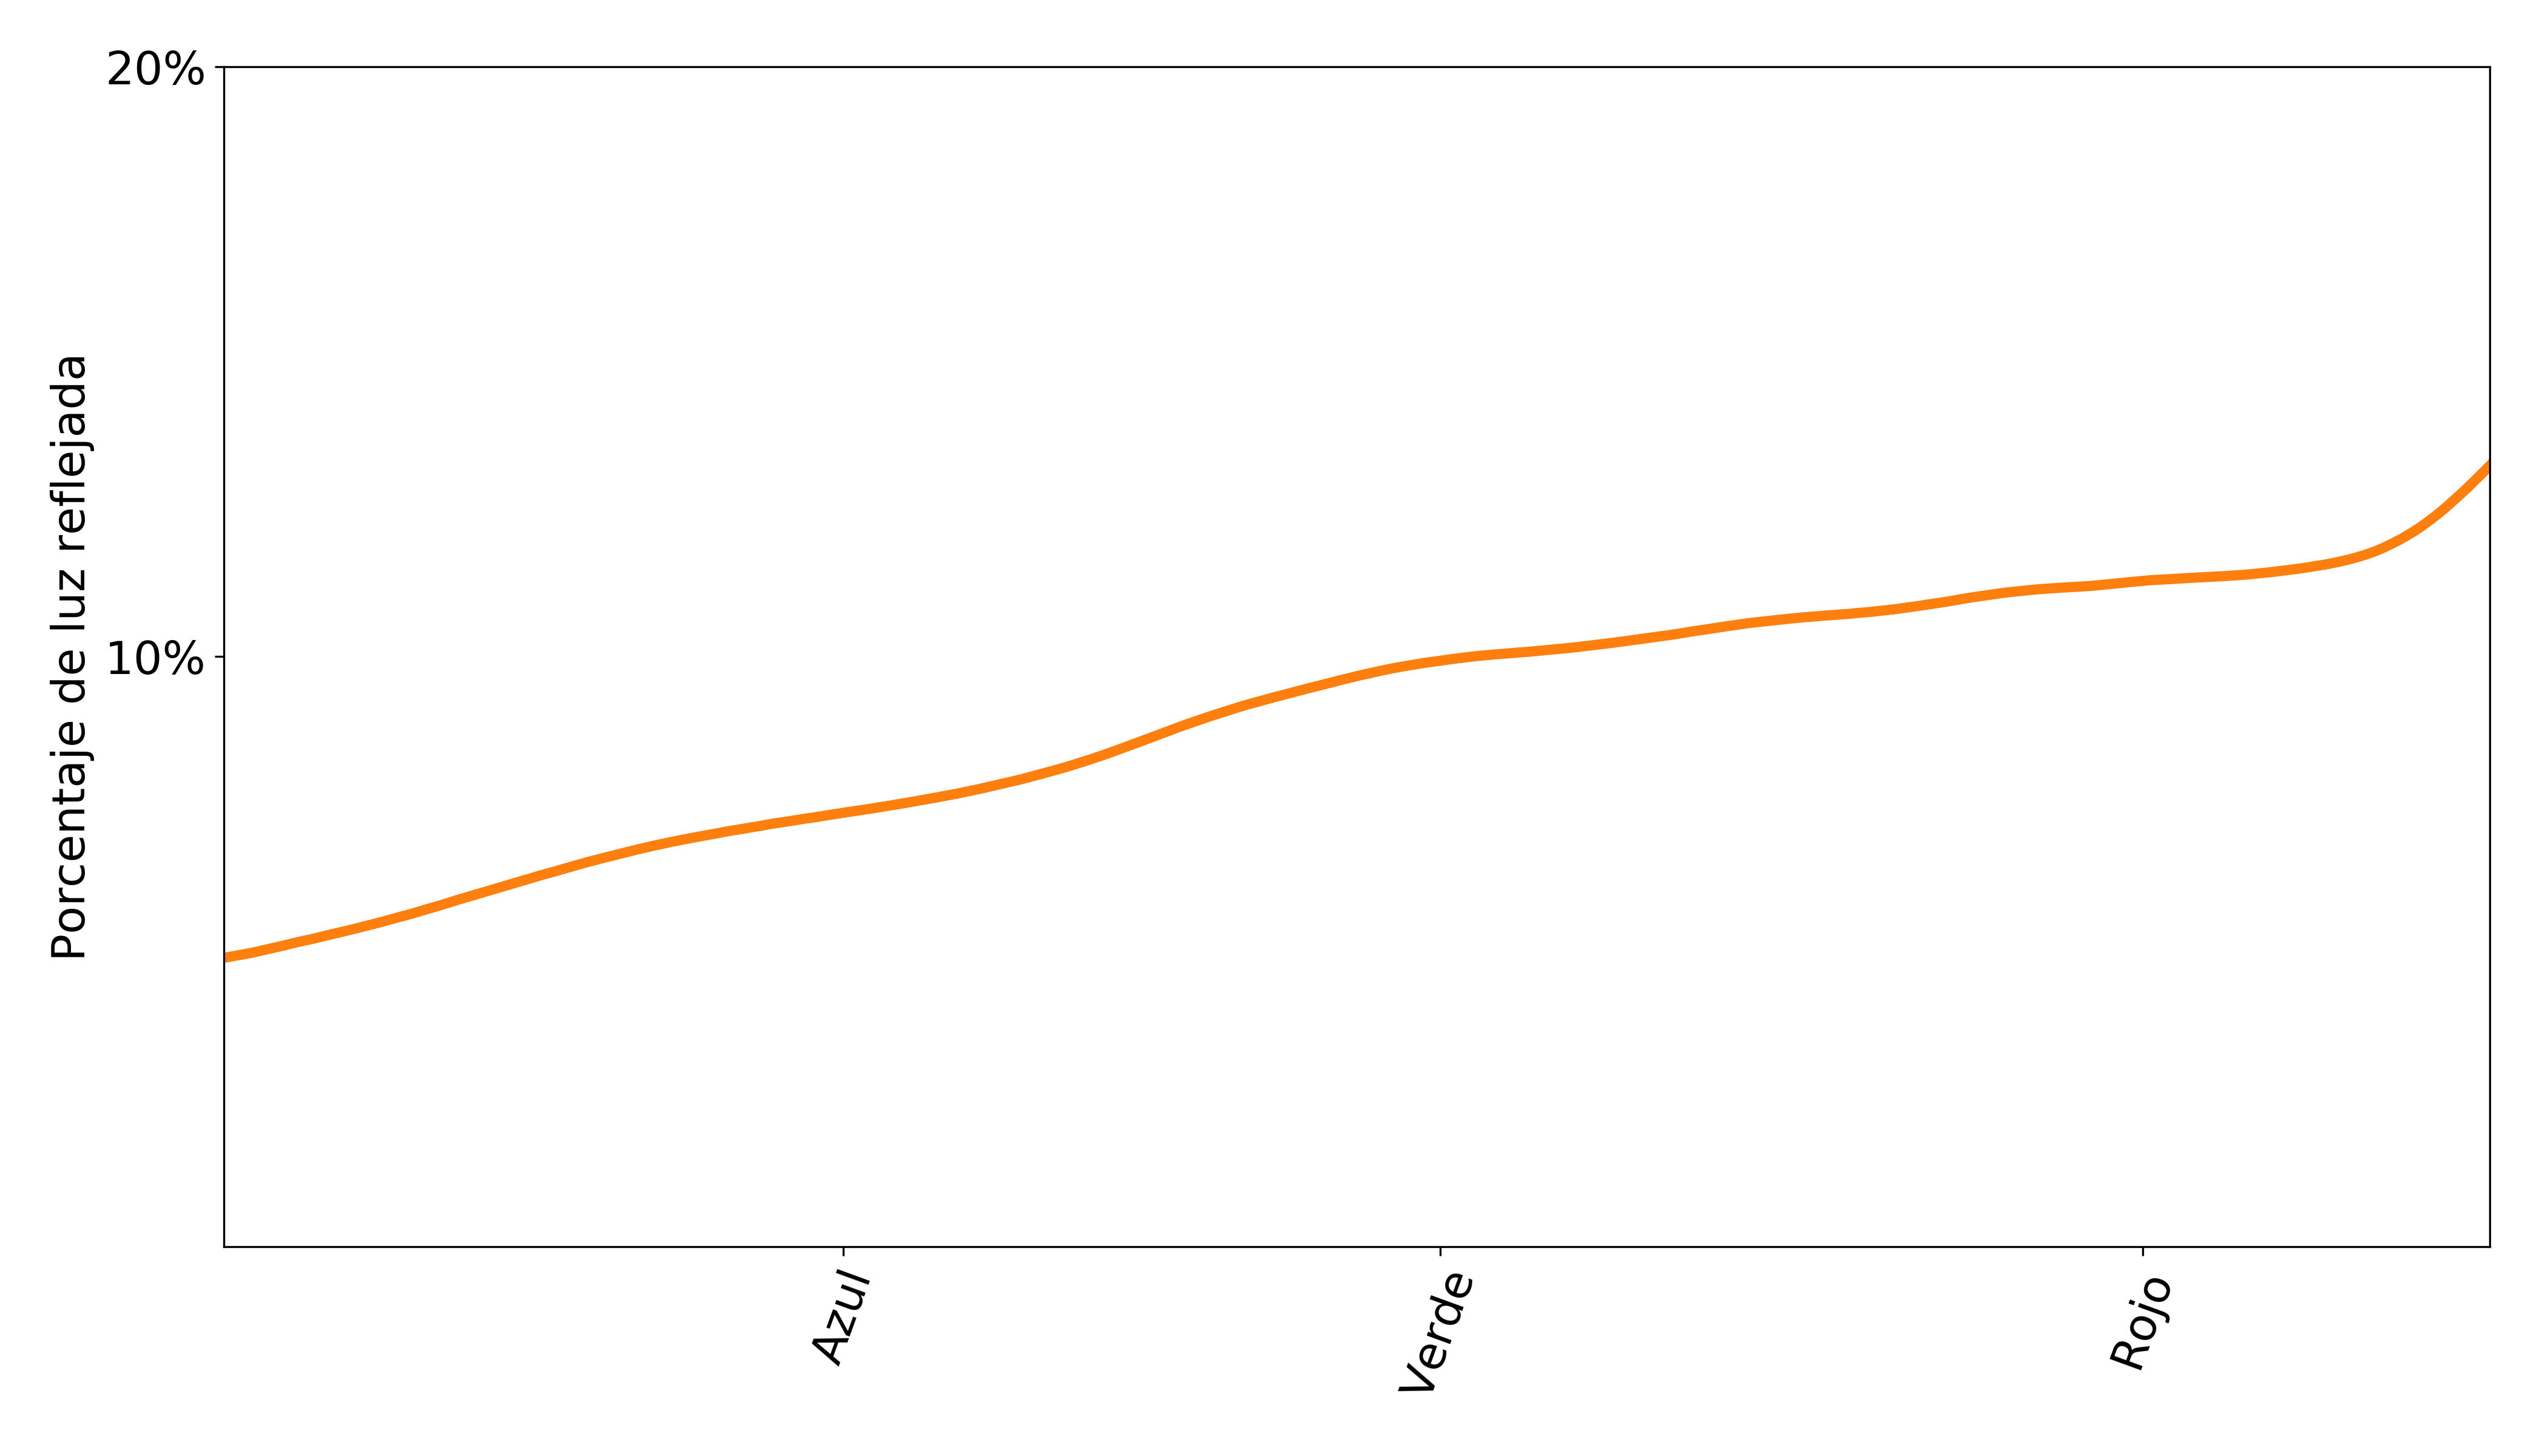
\includegraphics[width=0.8\textwidth]{fig:s.png}
    \caption{Firmas espectral de la suelo.}
    \label{}
  \end{figure}
\end{frame}
%--- Next Frame ---%

\begin{frame}{\secname : \subsecname}
  \begin{figure}
    \centering
    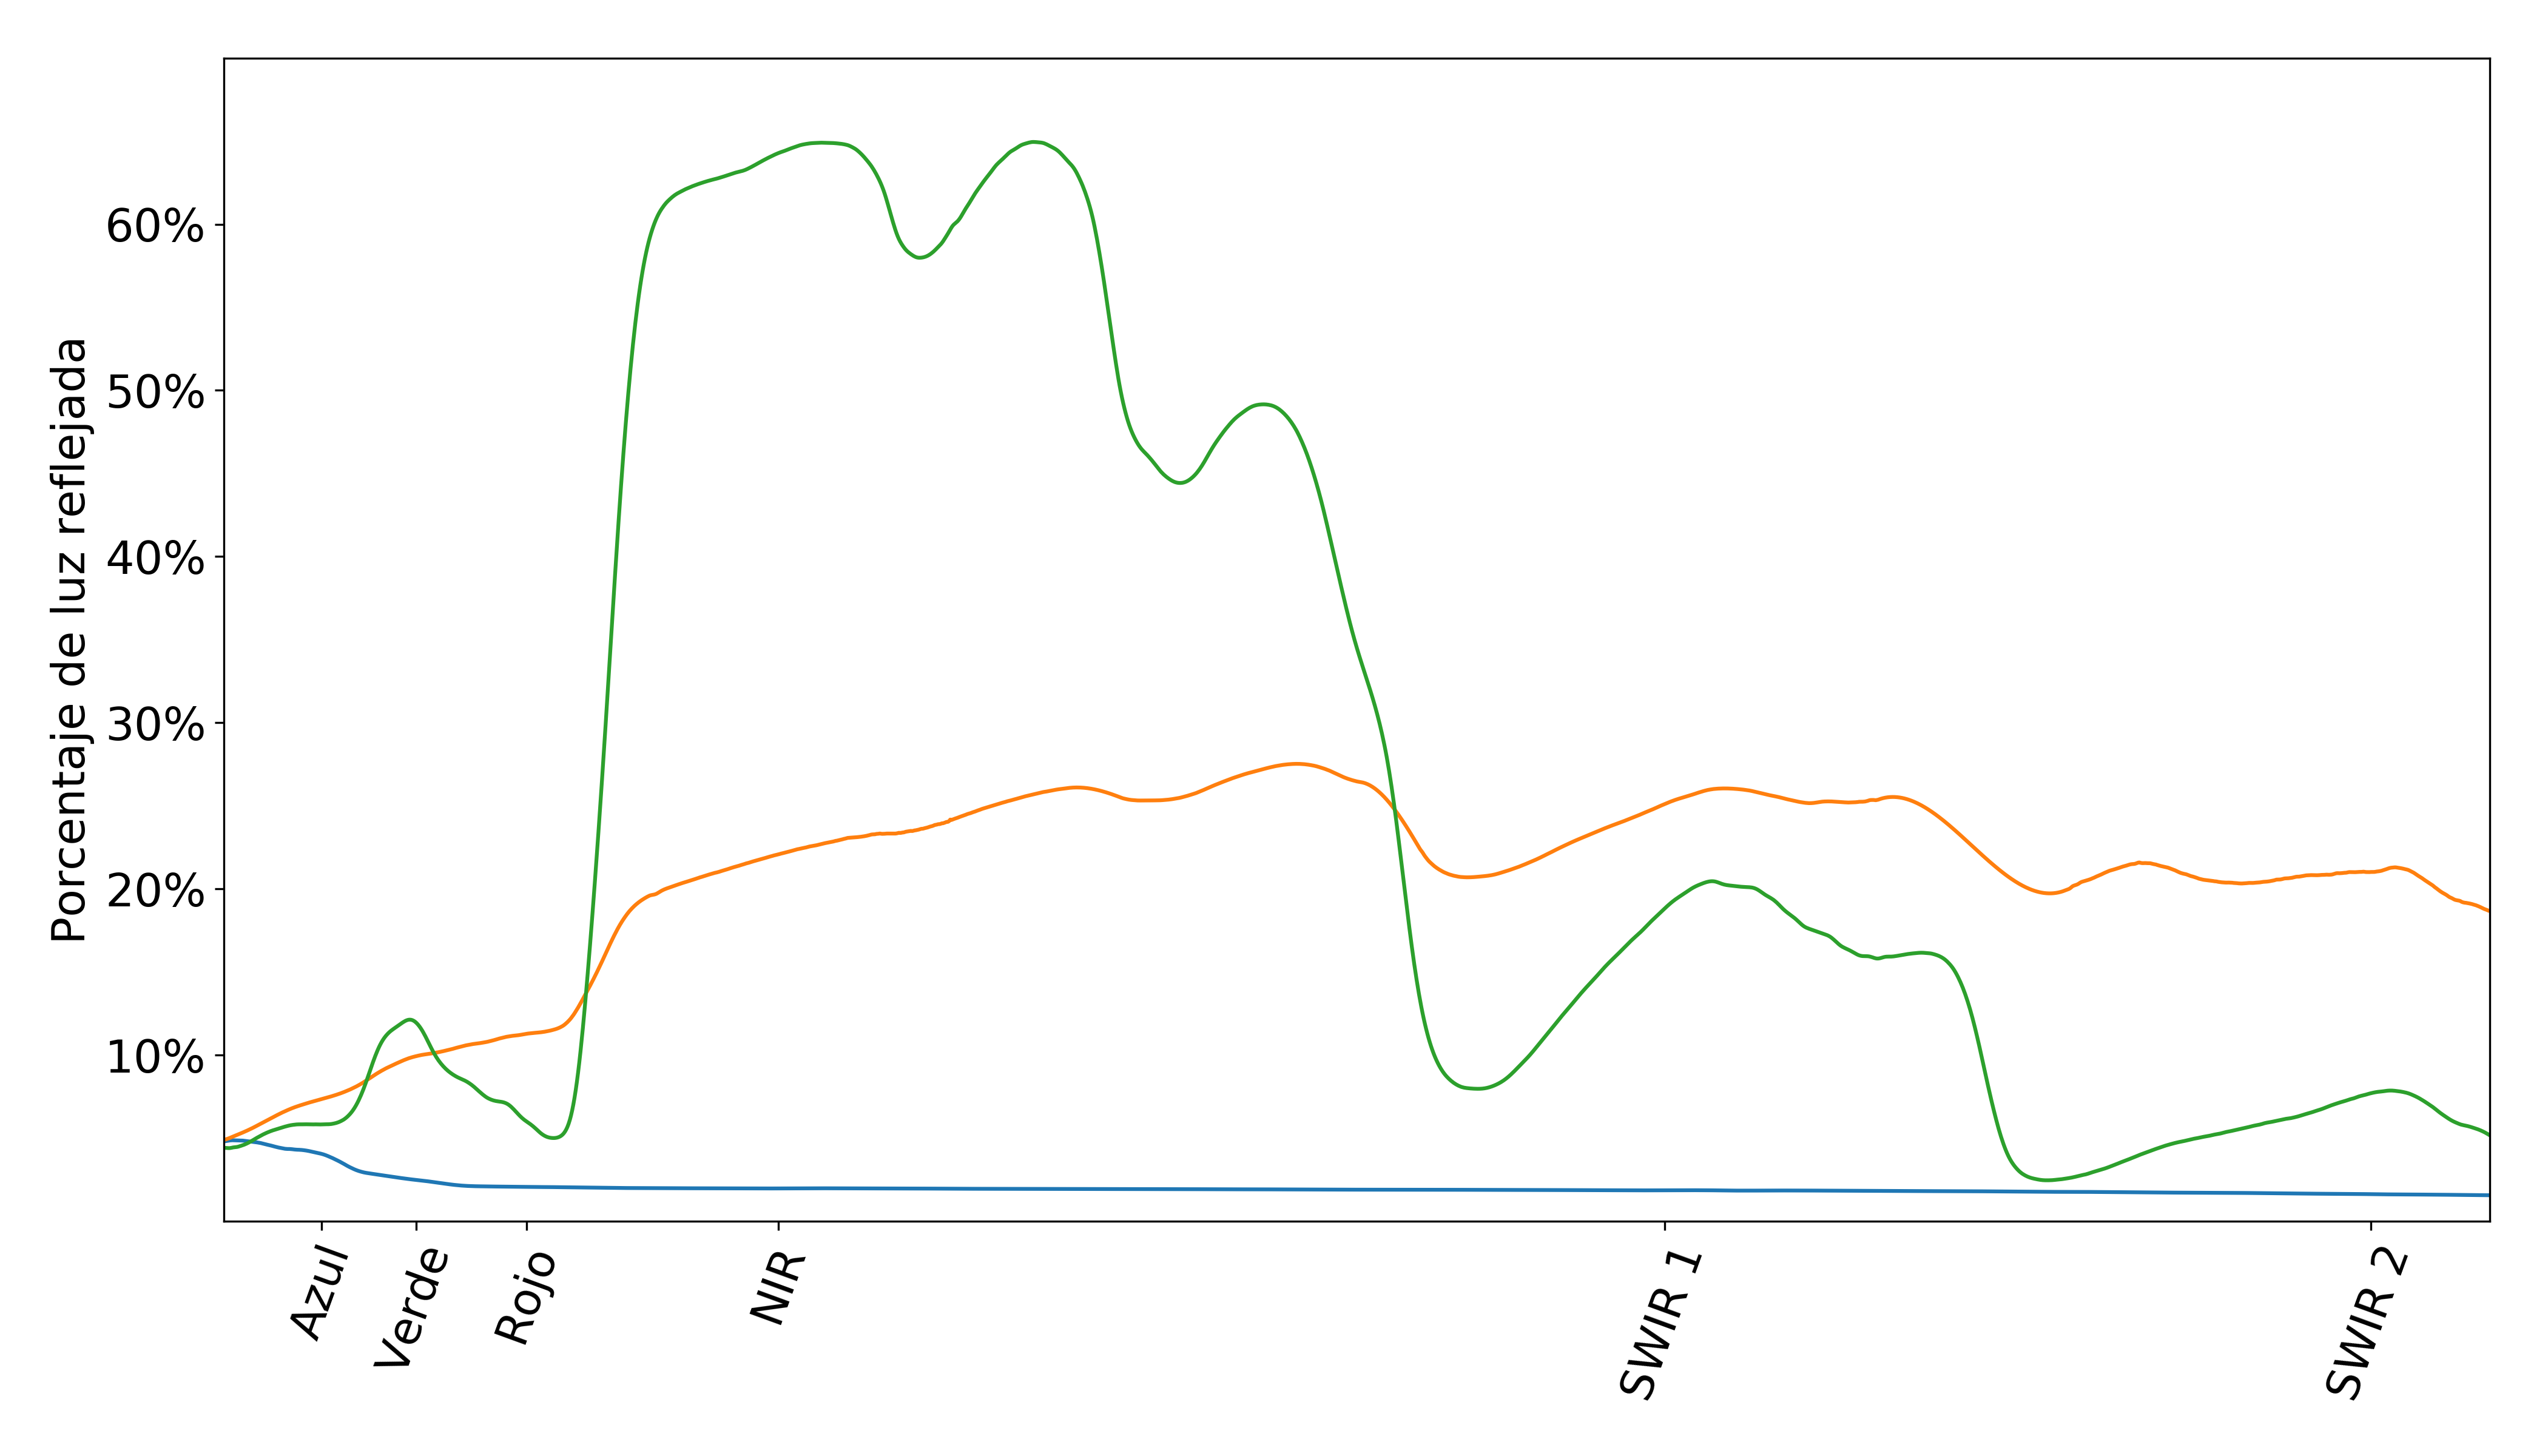
\includegraphics[width=0.8\textwidth]{fig:spec.png}
    \caption{Comparación de firmas espectrales..}
    \label{}
  \end{figure}
\end{frame}
%--- Next Frame ---%

\subsection{Interpretación visual}

\begin{frame}{\secname : \subsecname}
  \begin{figure}
    \centering
    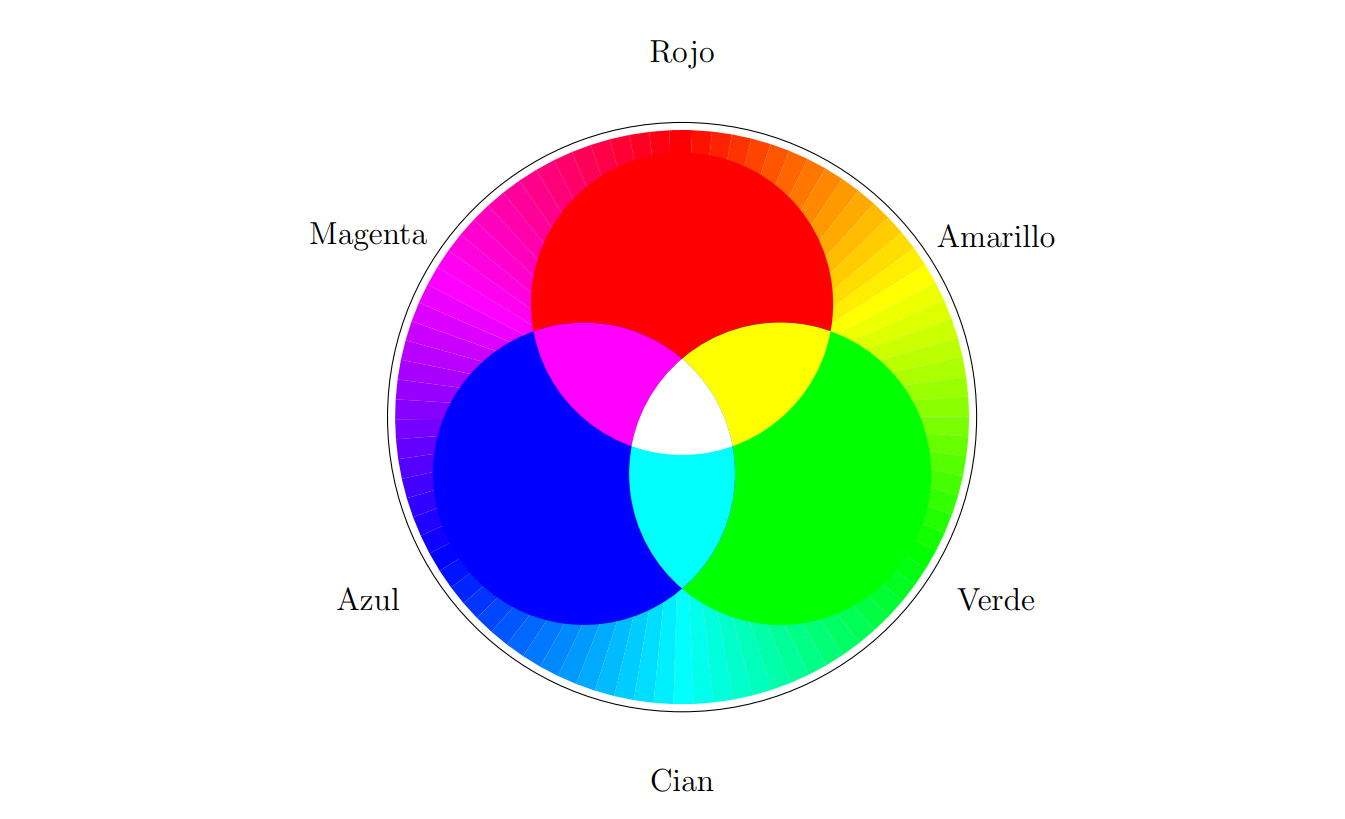
\includegraphics[width=0.45\textwidth]{fig:rgb.png}
    \caption{Teoría adivita del color.}
    \label{}
  \end{figure}
\end{frame}
%--- Next Frame ---%

\begin{frame}{\secname : \subsecname}
  \begin{figure}
    \centering
    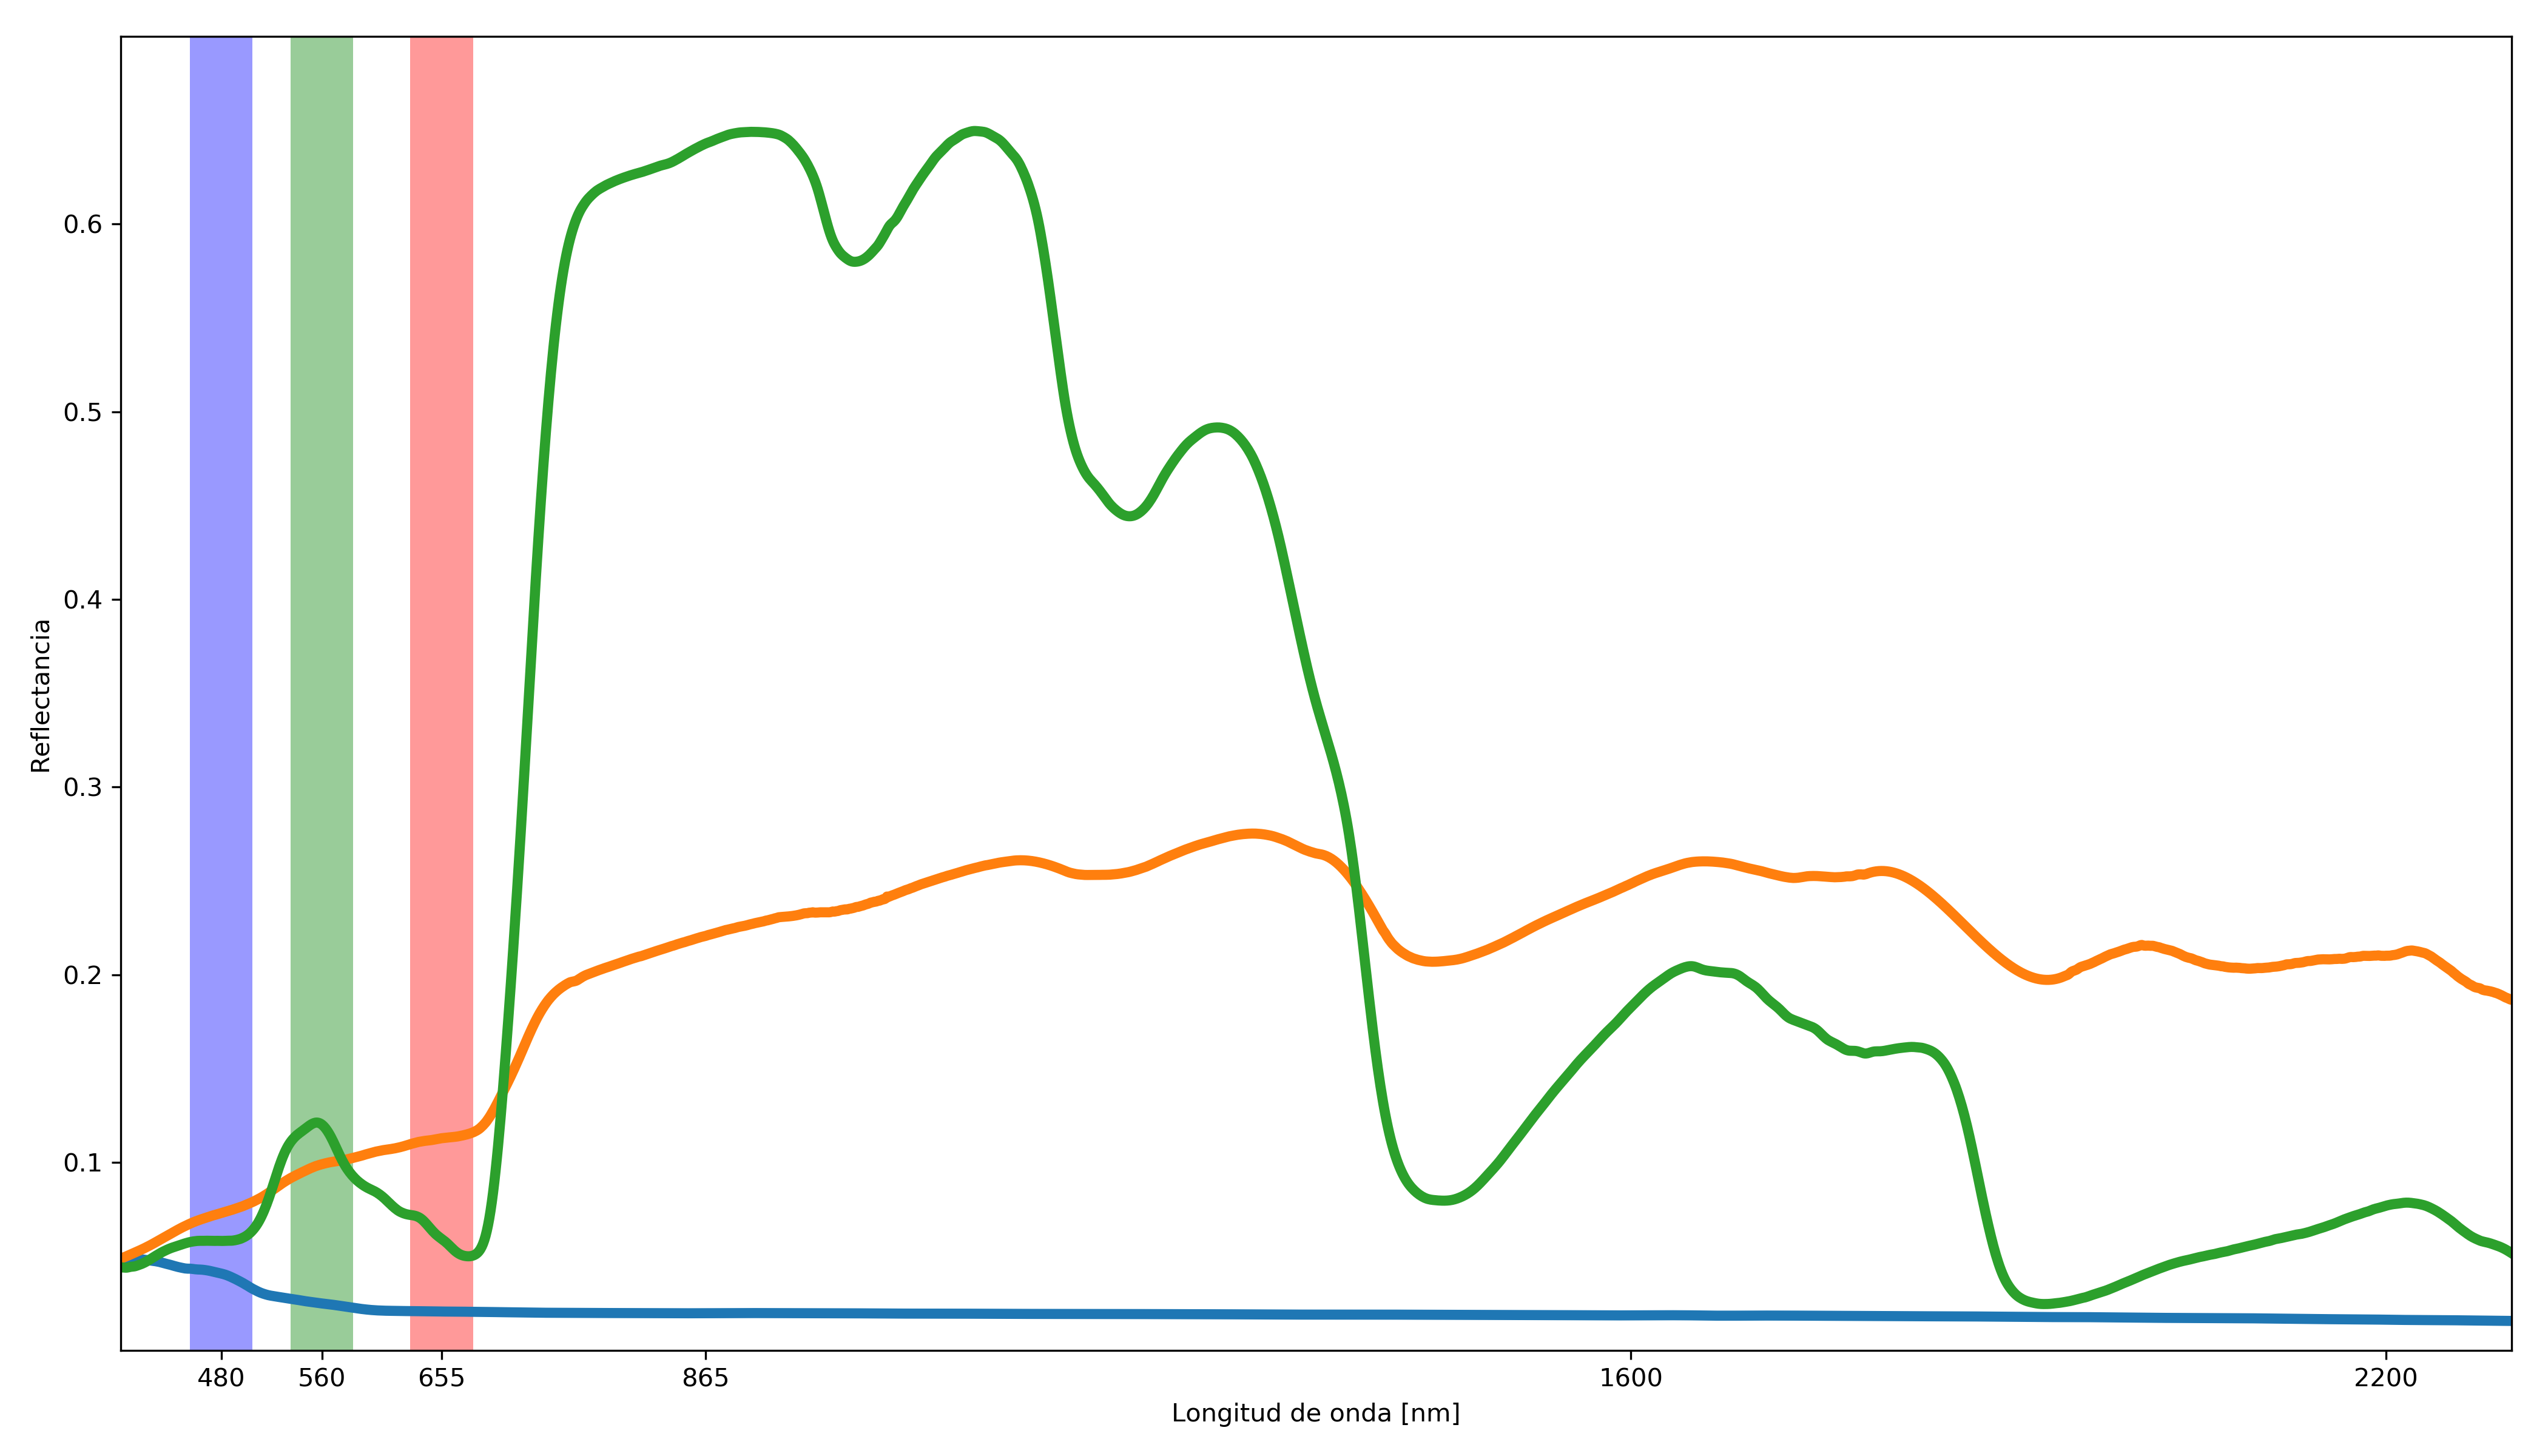
\includegraphics[width=0.8\textwidth]{fig:esreal.png}
    \caption{Interpretación visual - color real. }
    \label{}
  \end{figure}
\end{frame}
%--- Next Frame ---%

\begin{frame}{\secname : \subsecname}
  \begin{figure}
    \centering
    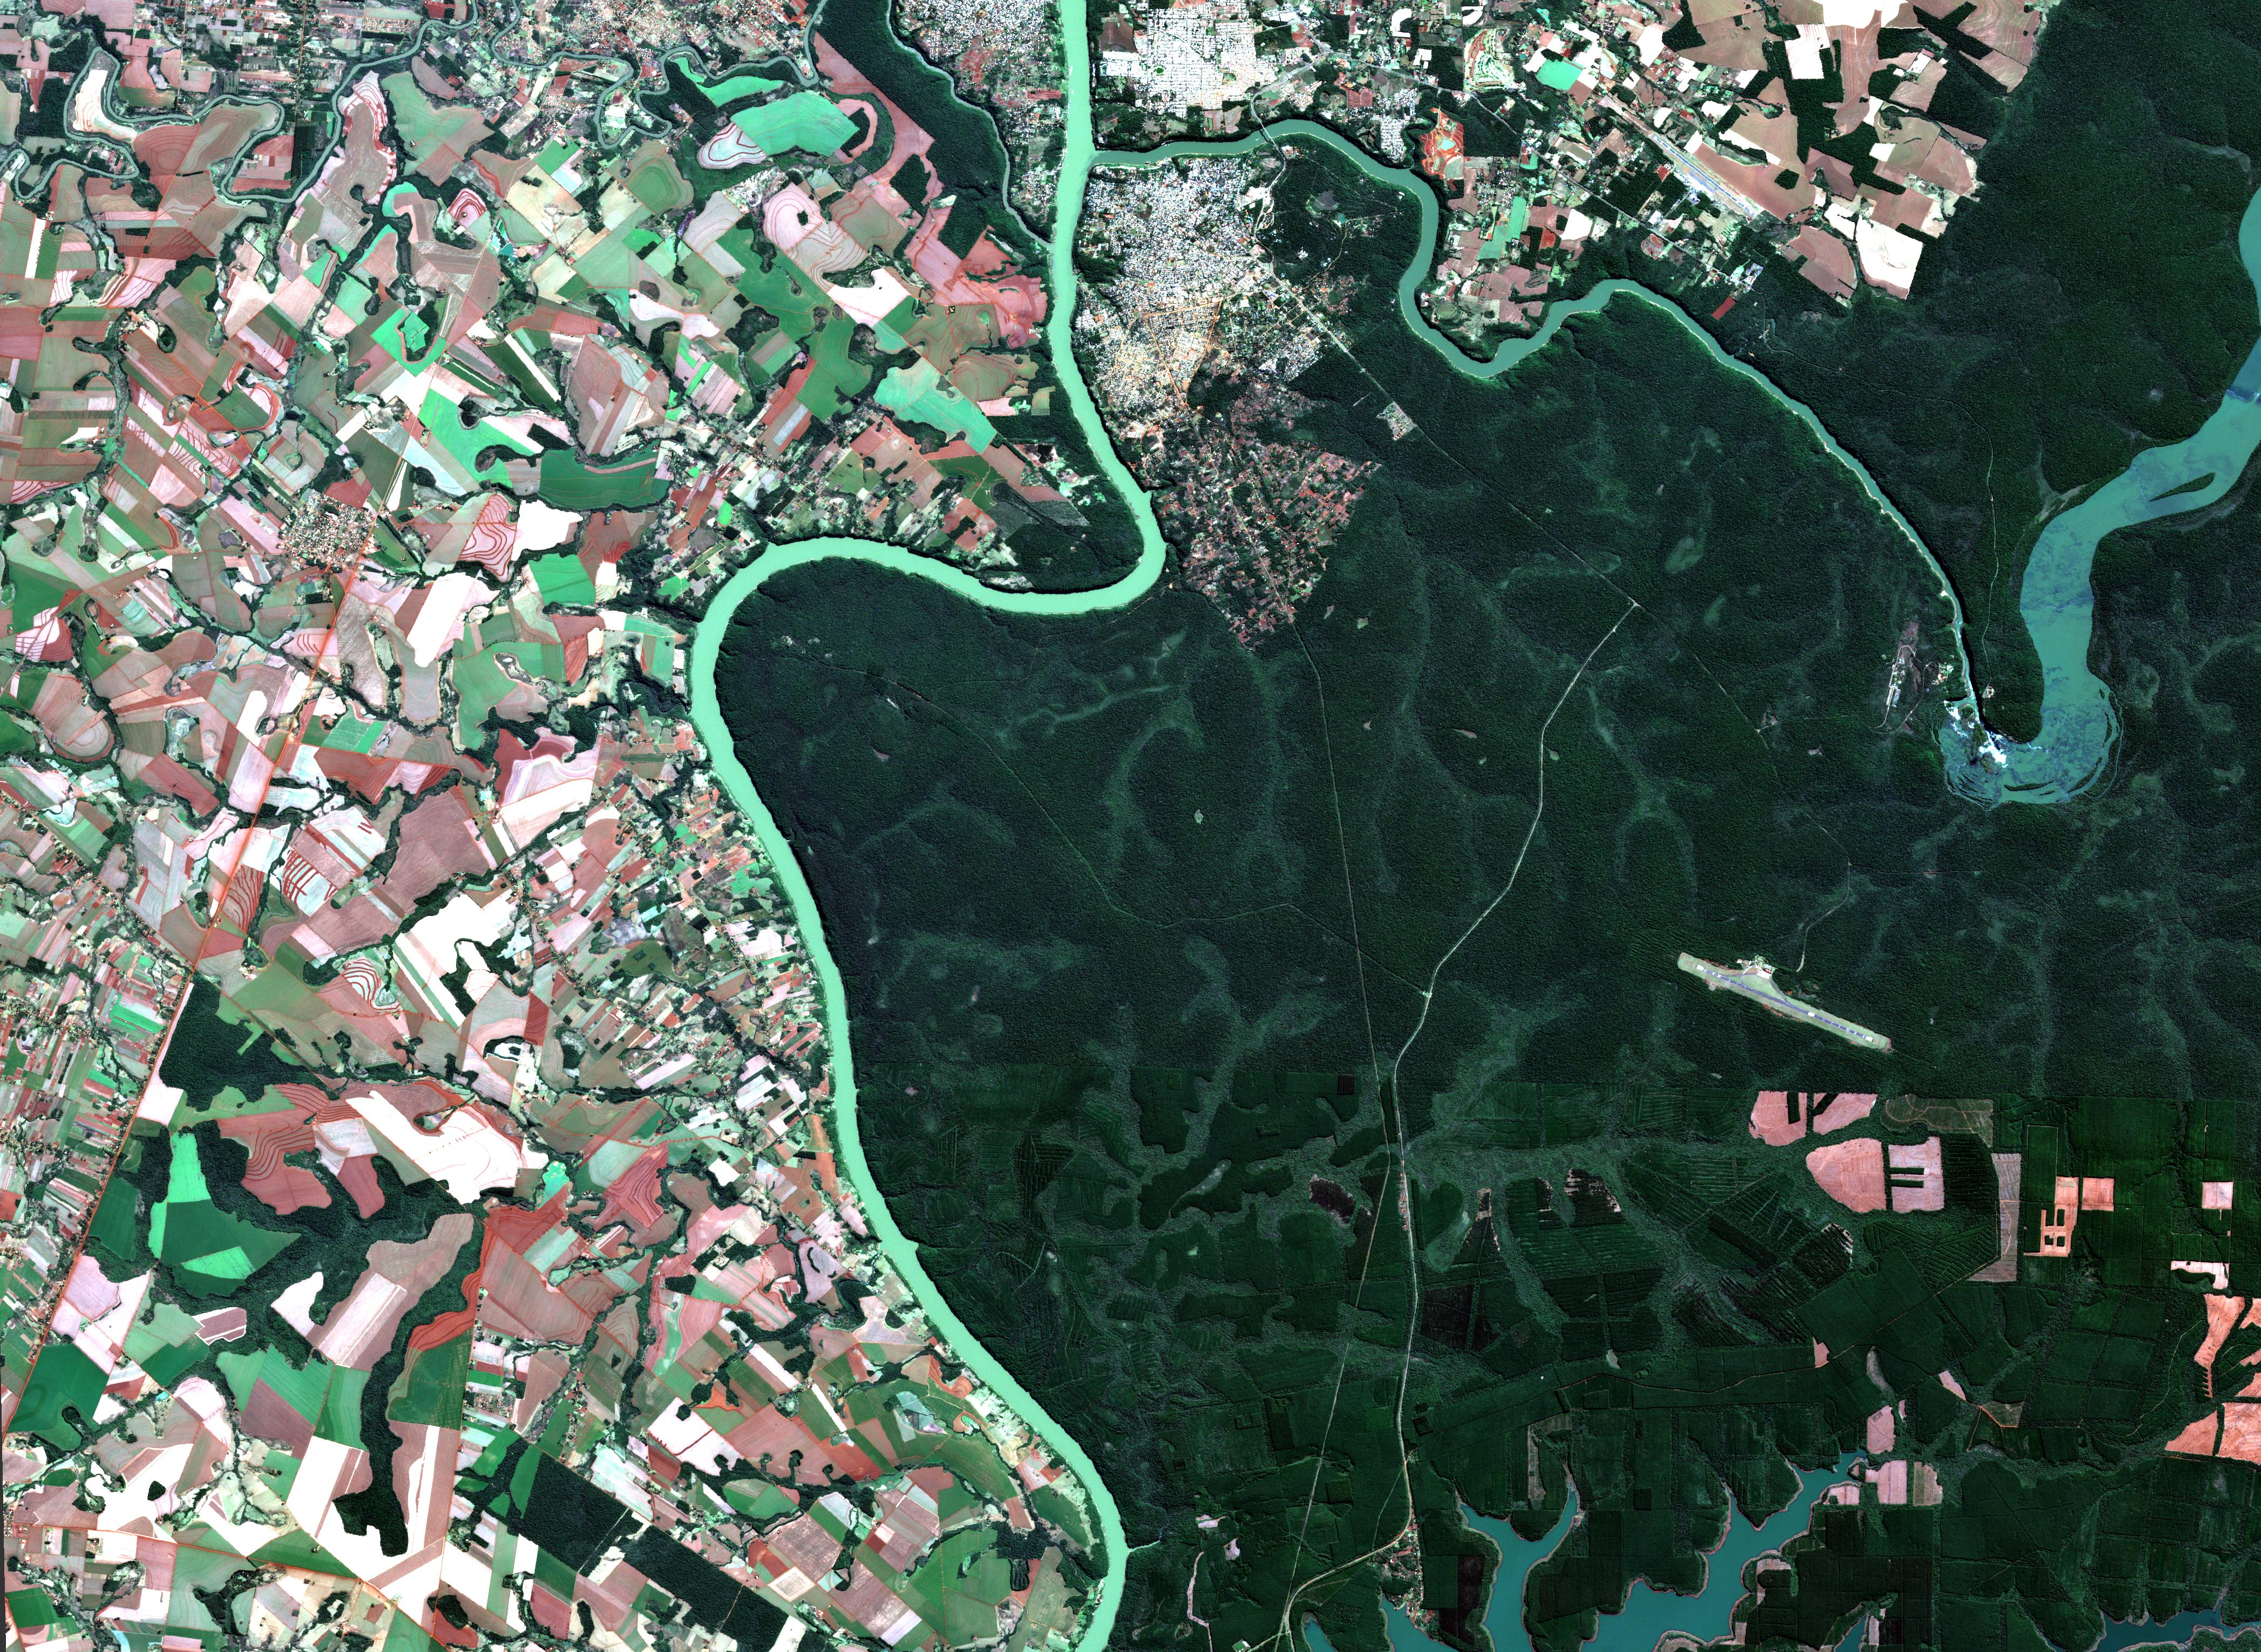
\includegraphics[width=0.6\textwidth]{fig:imreal.jpeg}
    \caption{Interpretación visual - color real.}
    \label{}
  \end{figure}
\end{frame}
%--- Next Frame ---%

\begin{frame}{\secname : \subsecname}
  \begin{figure}
    \centering
    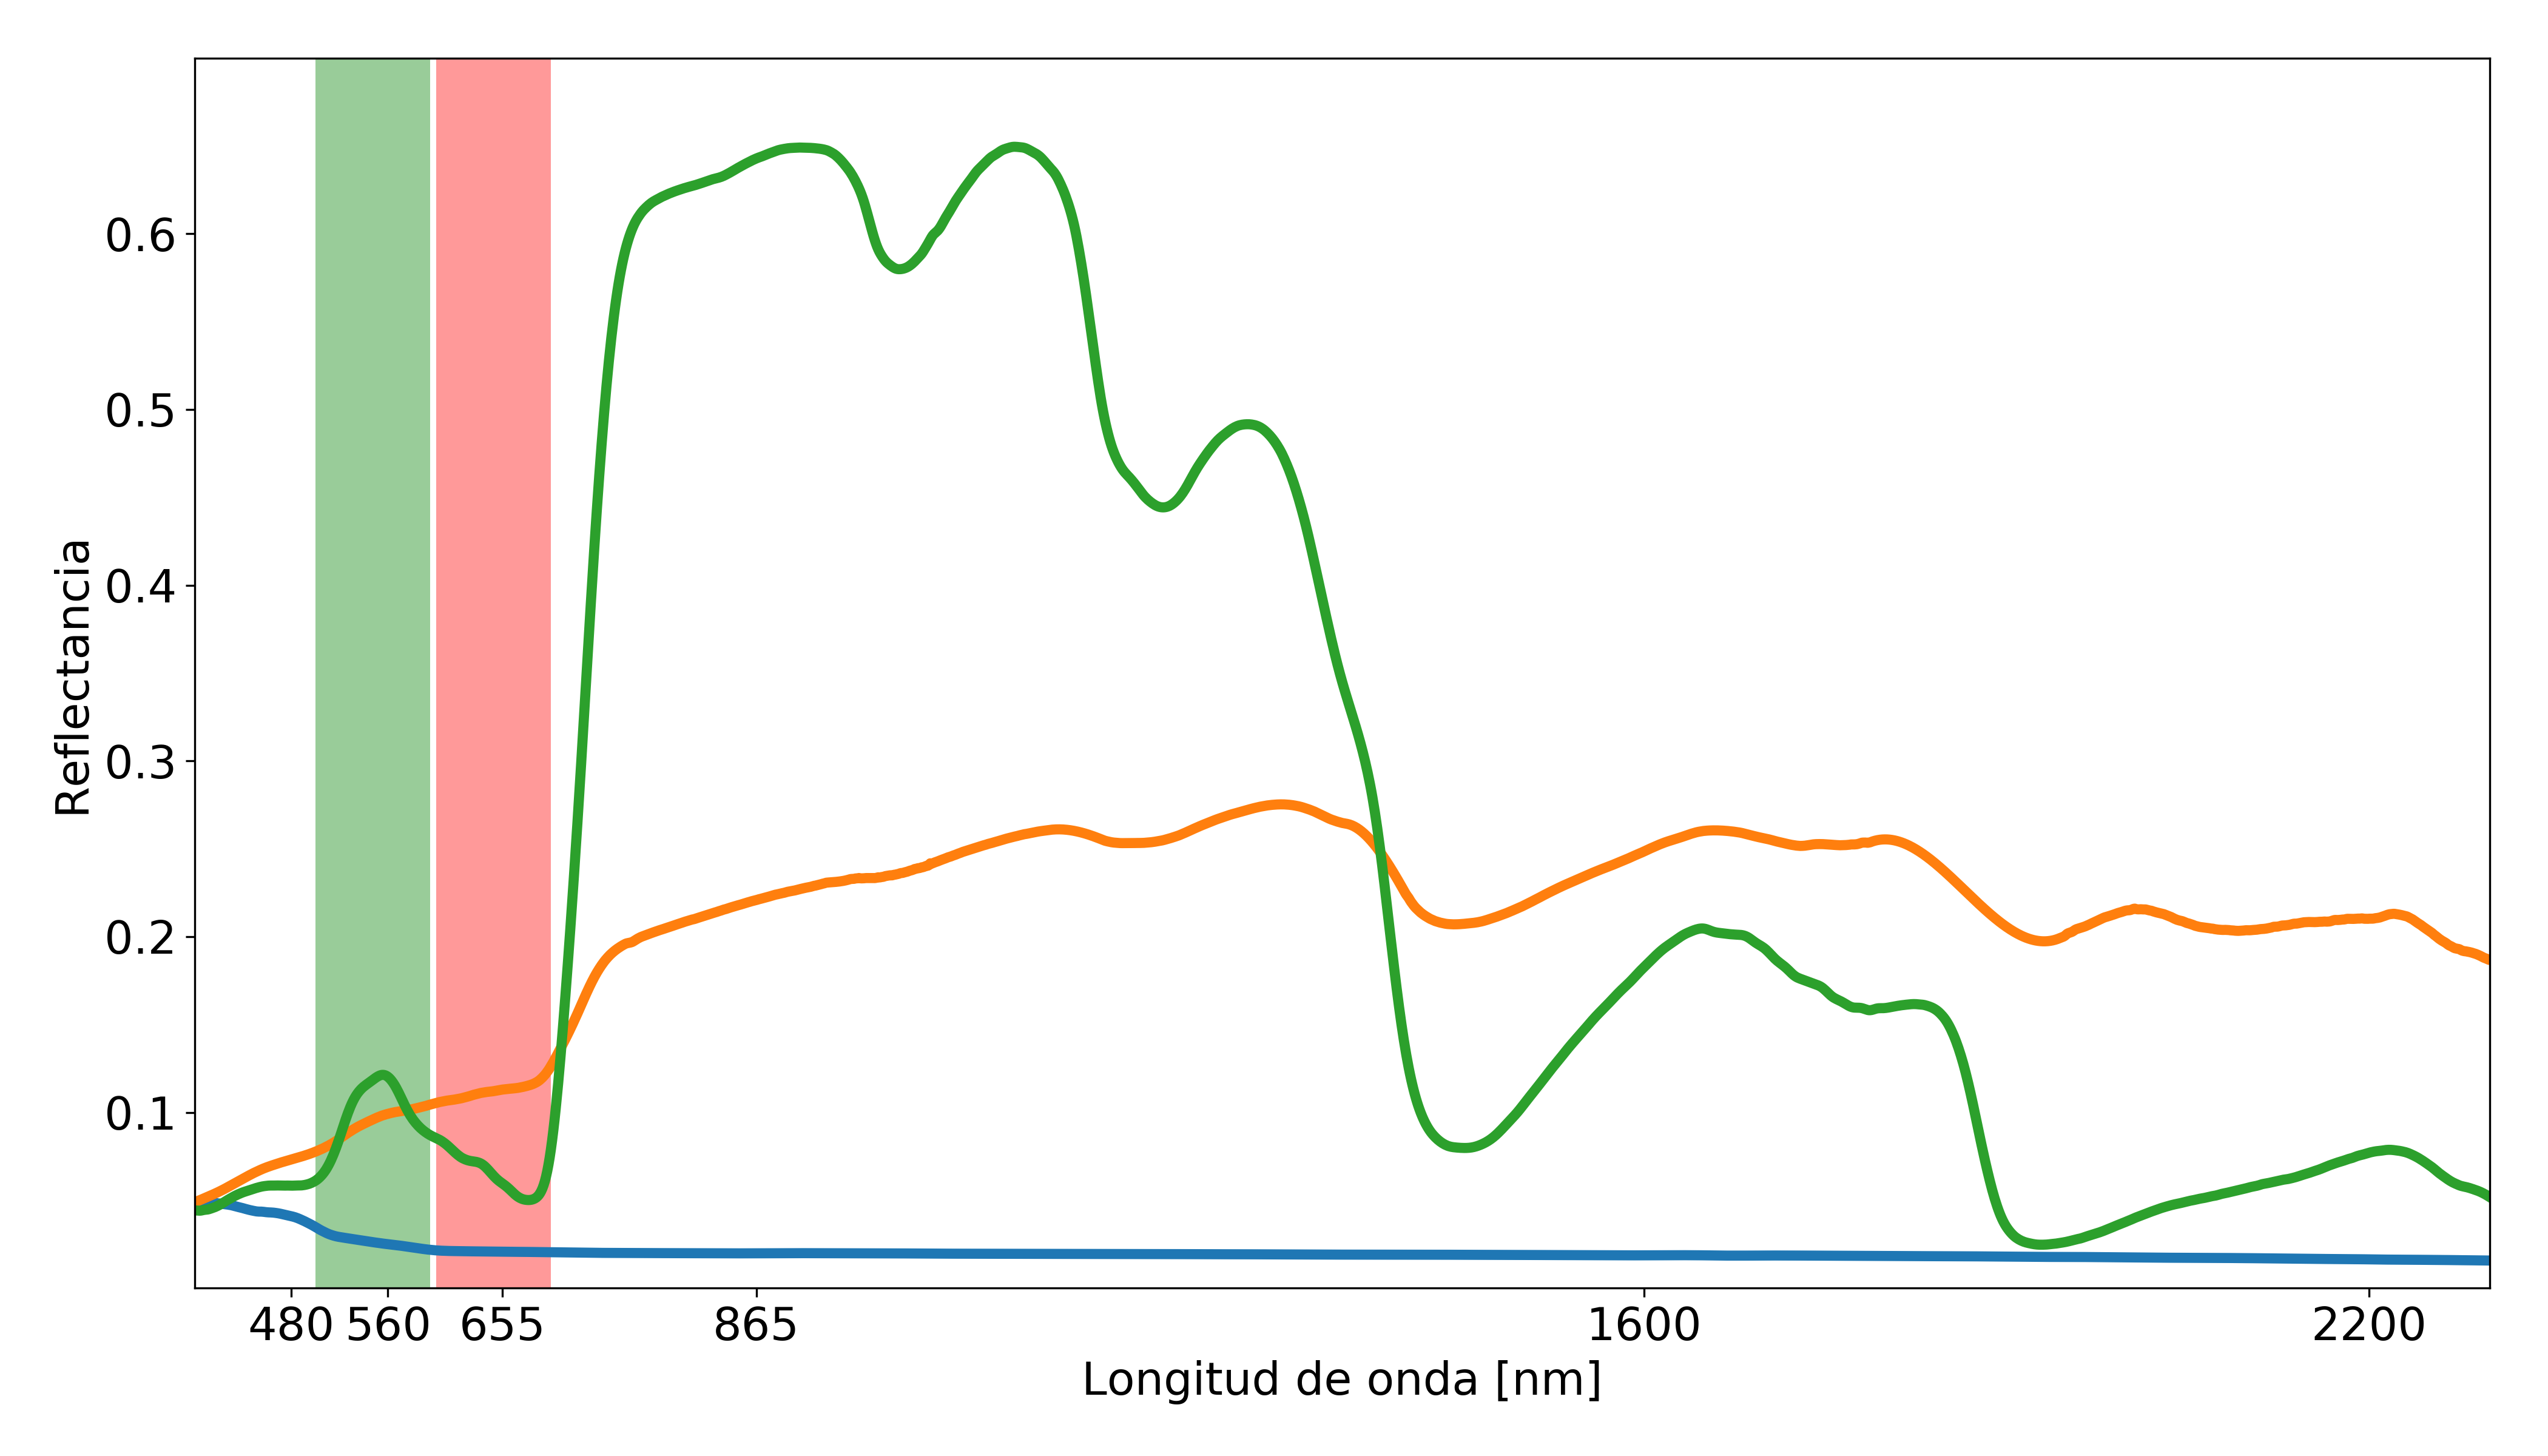
\includegraphics[width=0.8\textwidth]{fig:esinfra.png}
    \caption{Interpretación visual - infrarrojo color.}
    \label{}
  \end{figure}
\end{frame}
%--- Next Frame ---%

\begin{frame}{\secname : \subsecname}
  \begin{figure}
    \centering
    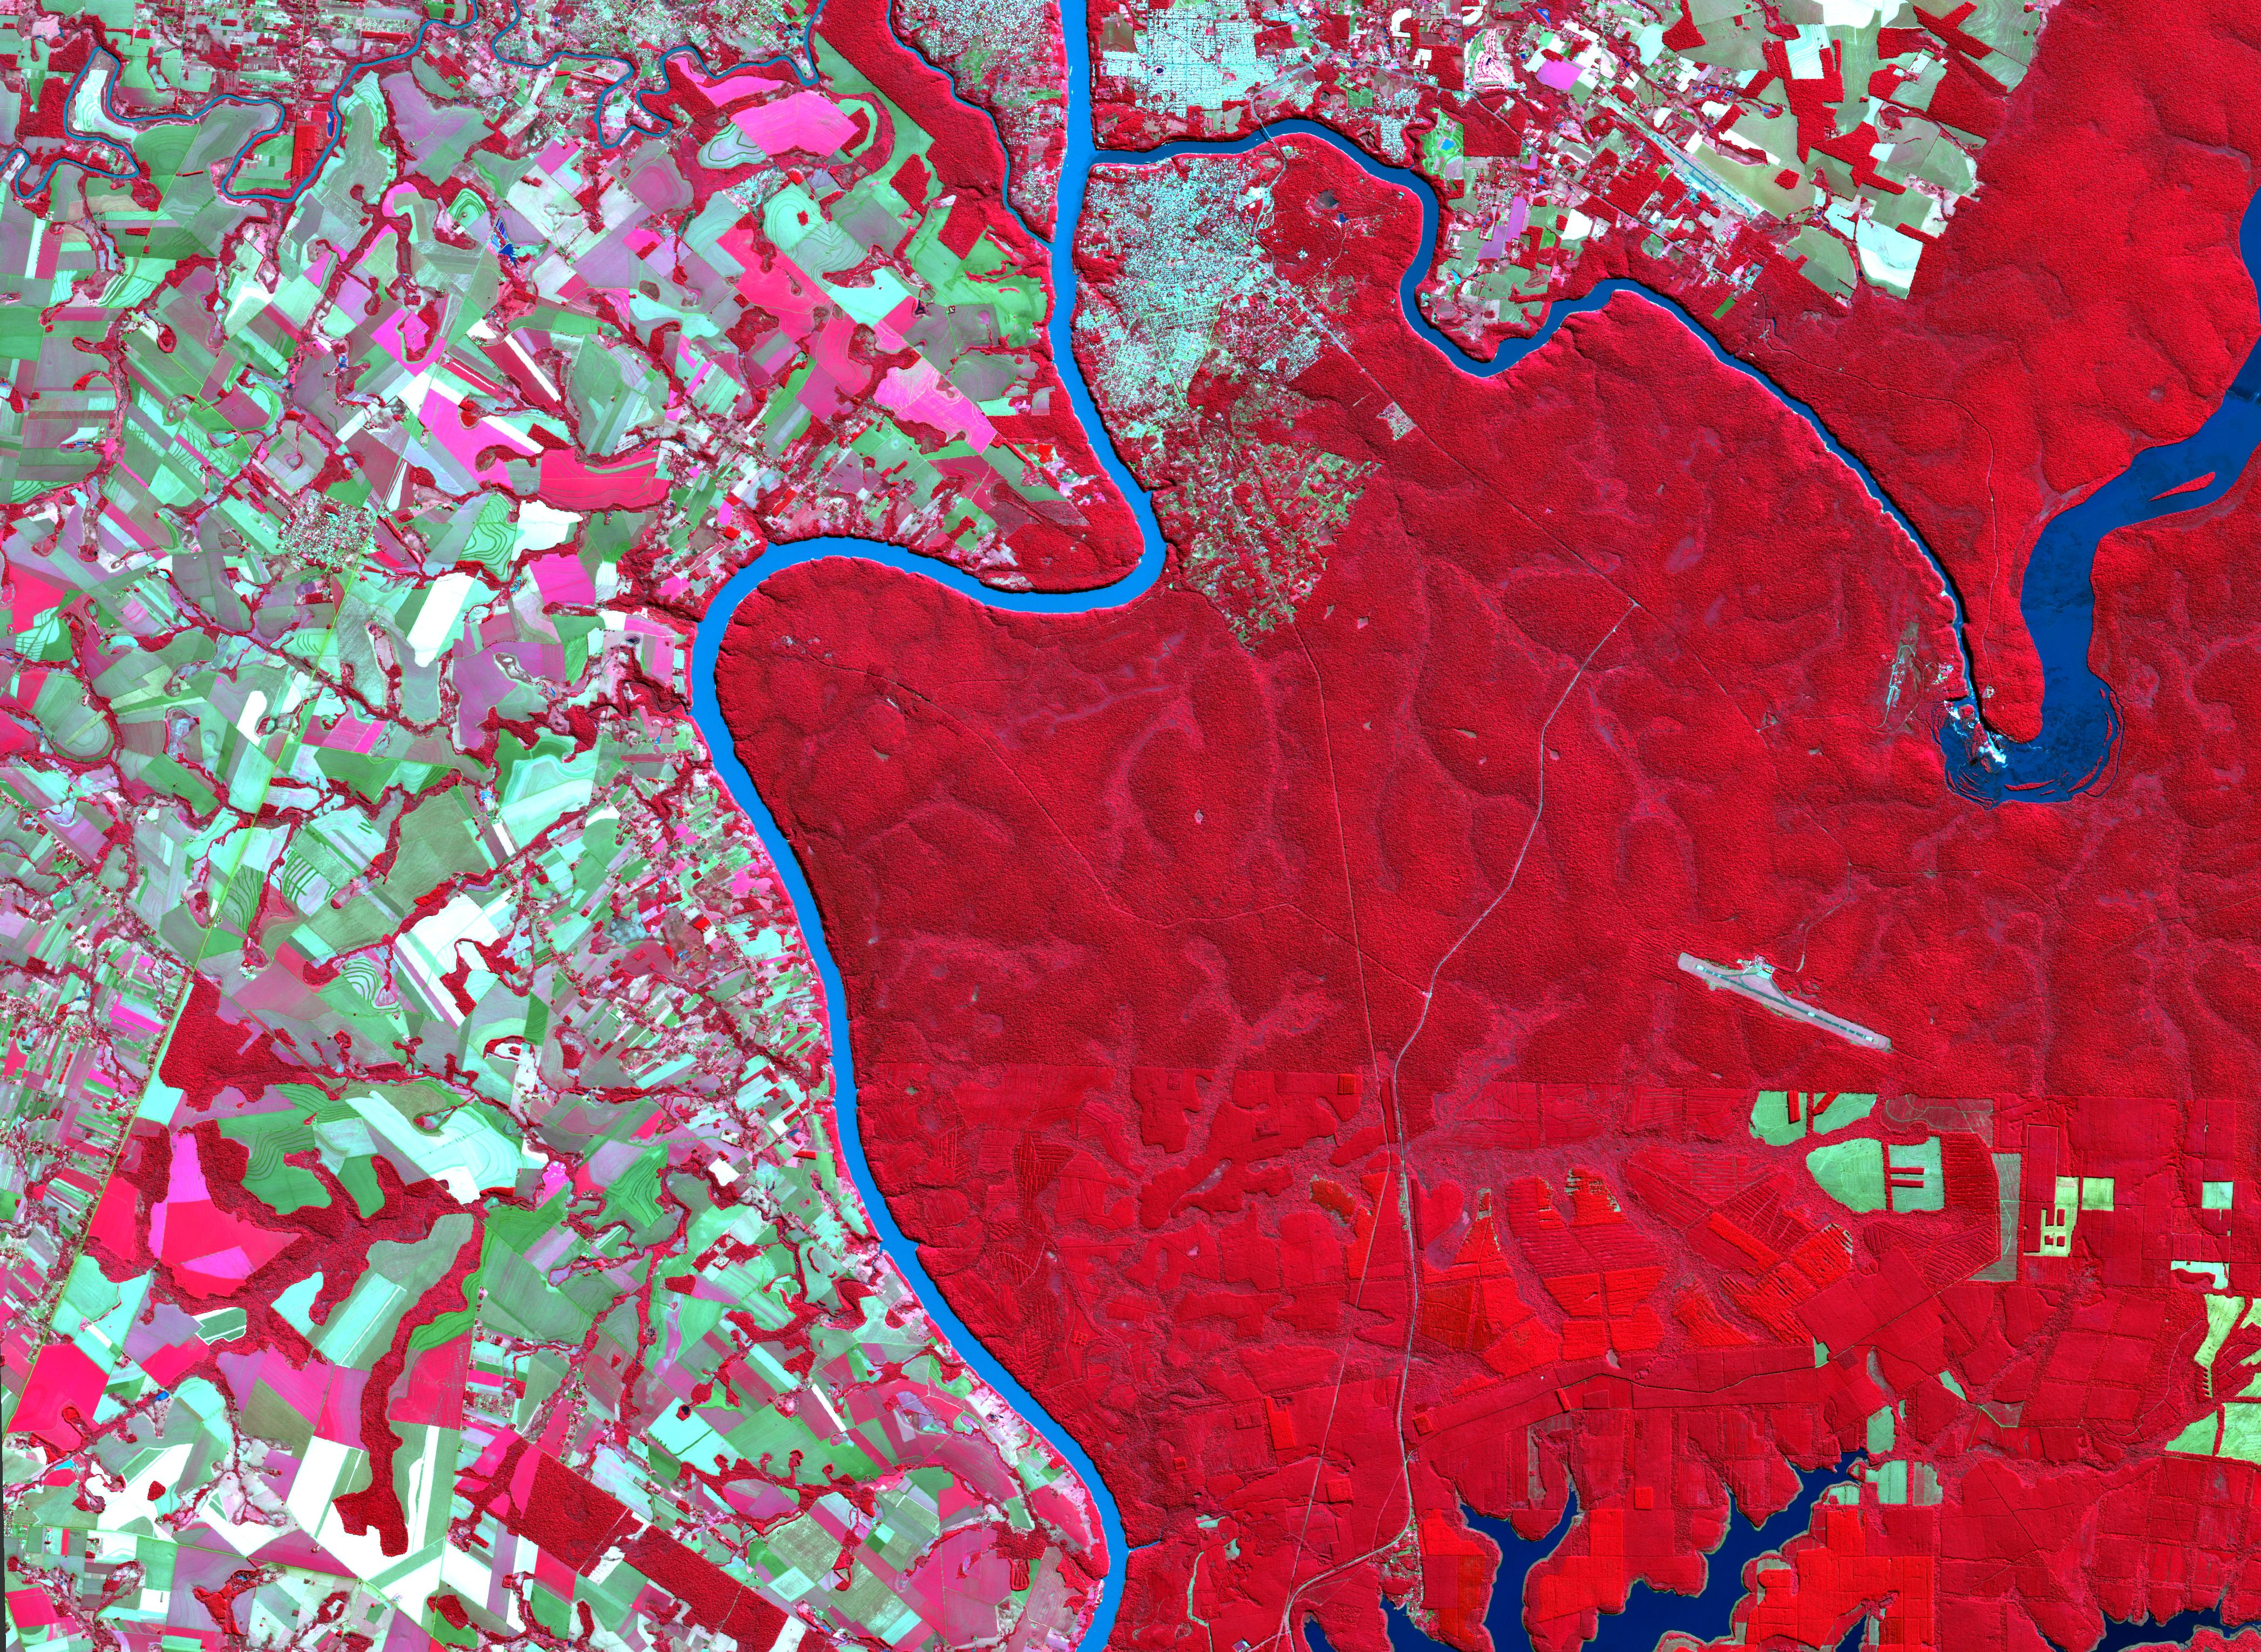
\includegraphics[width=0.6\textwidth]{fig:iminfra.jpeg}
    \caption{Interpretación visual - infrarrojo color.}
    \label{}
  \end{figure}
\end{frame}
%--- Next Frame ---%

\begin{frame}{\secname : \subsecname}
  \begin{figure}
    \centering
    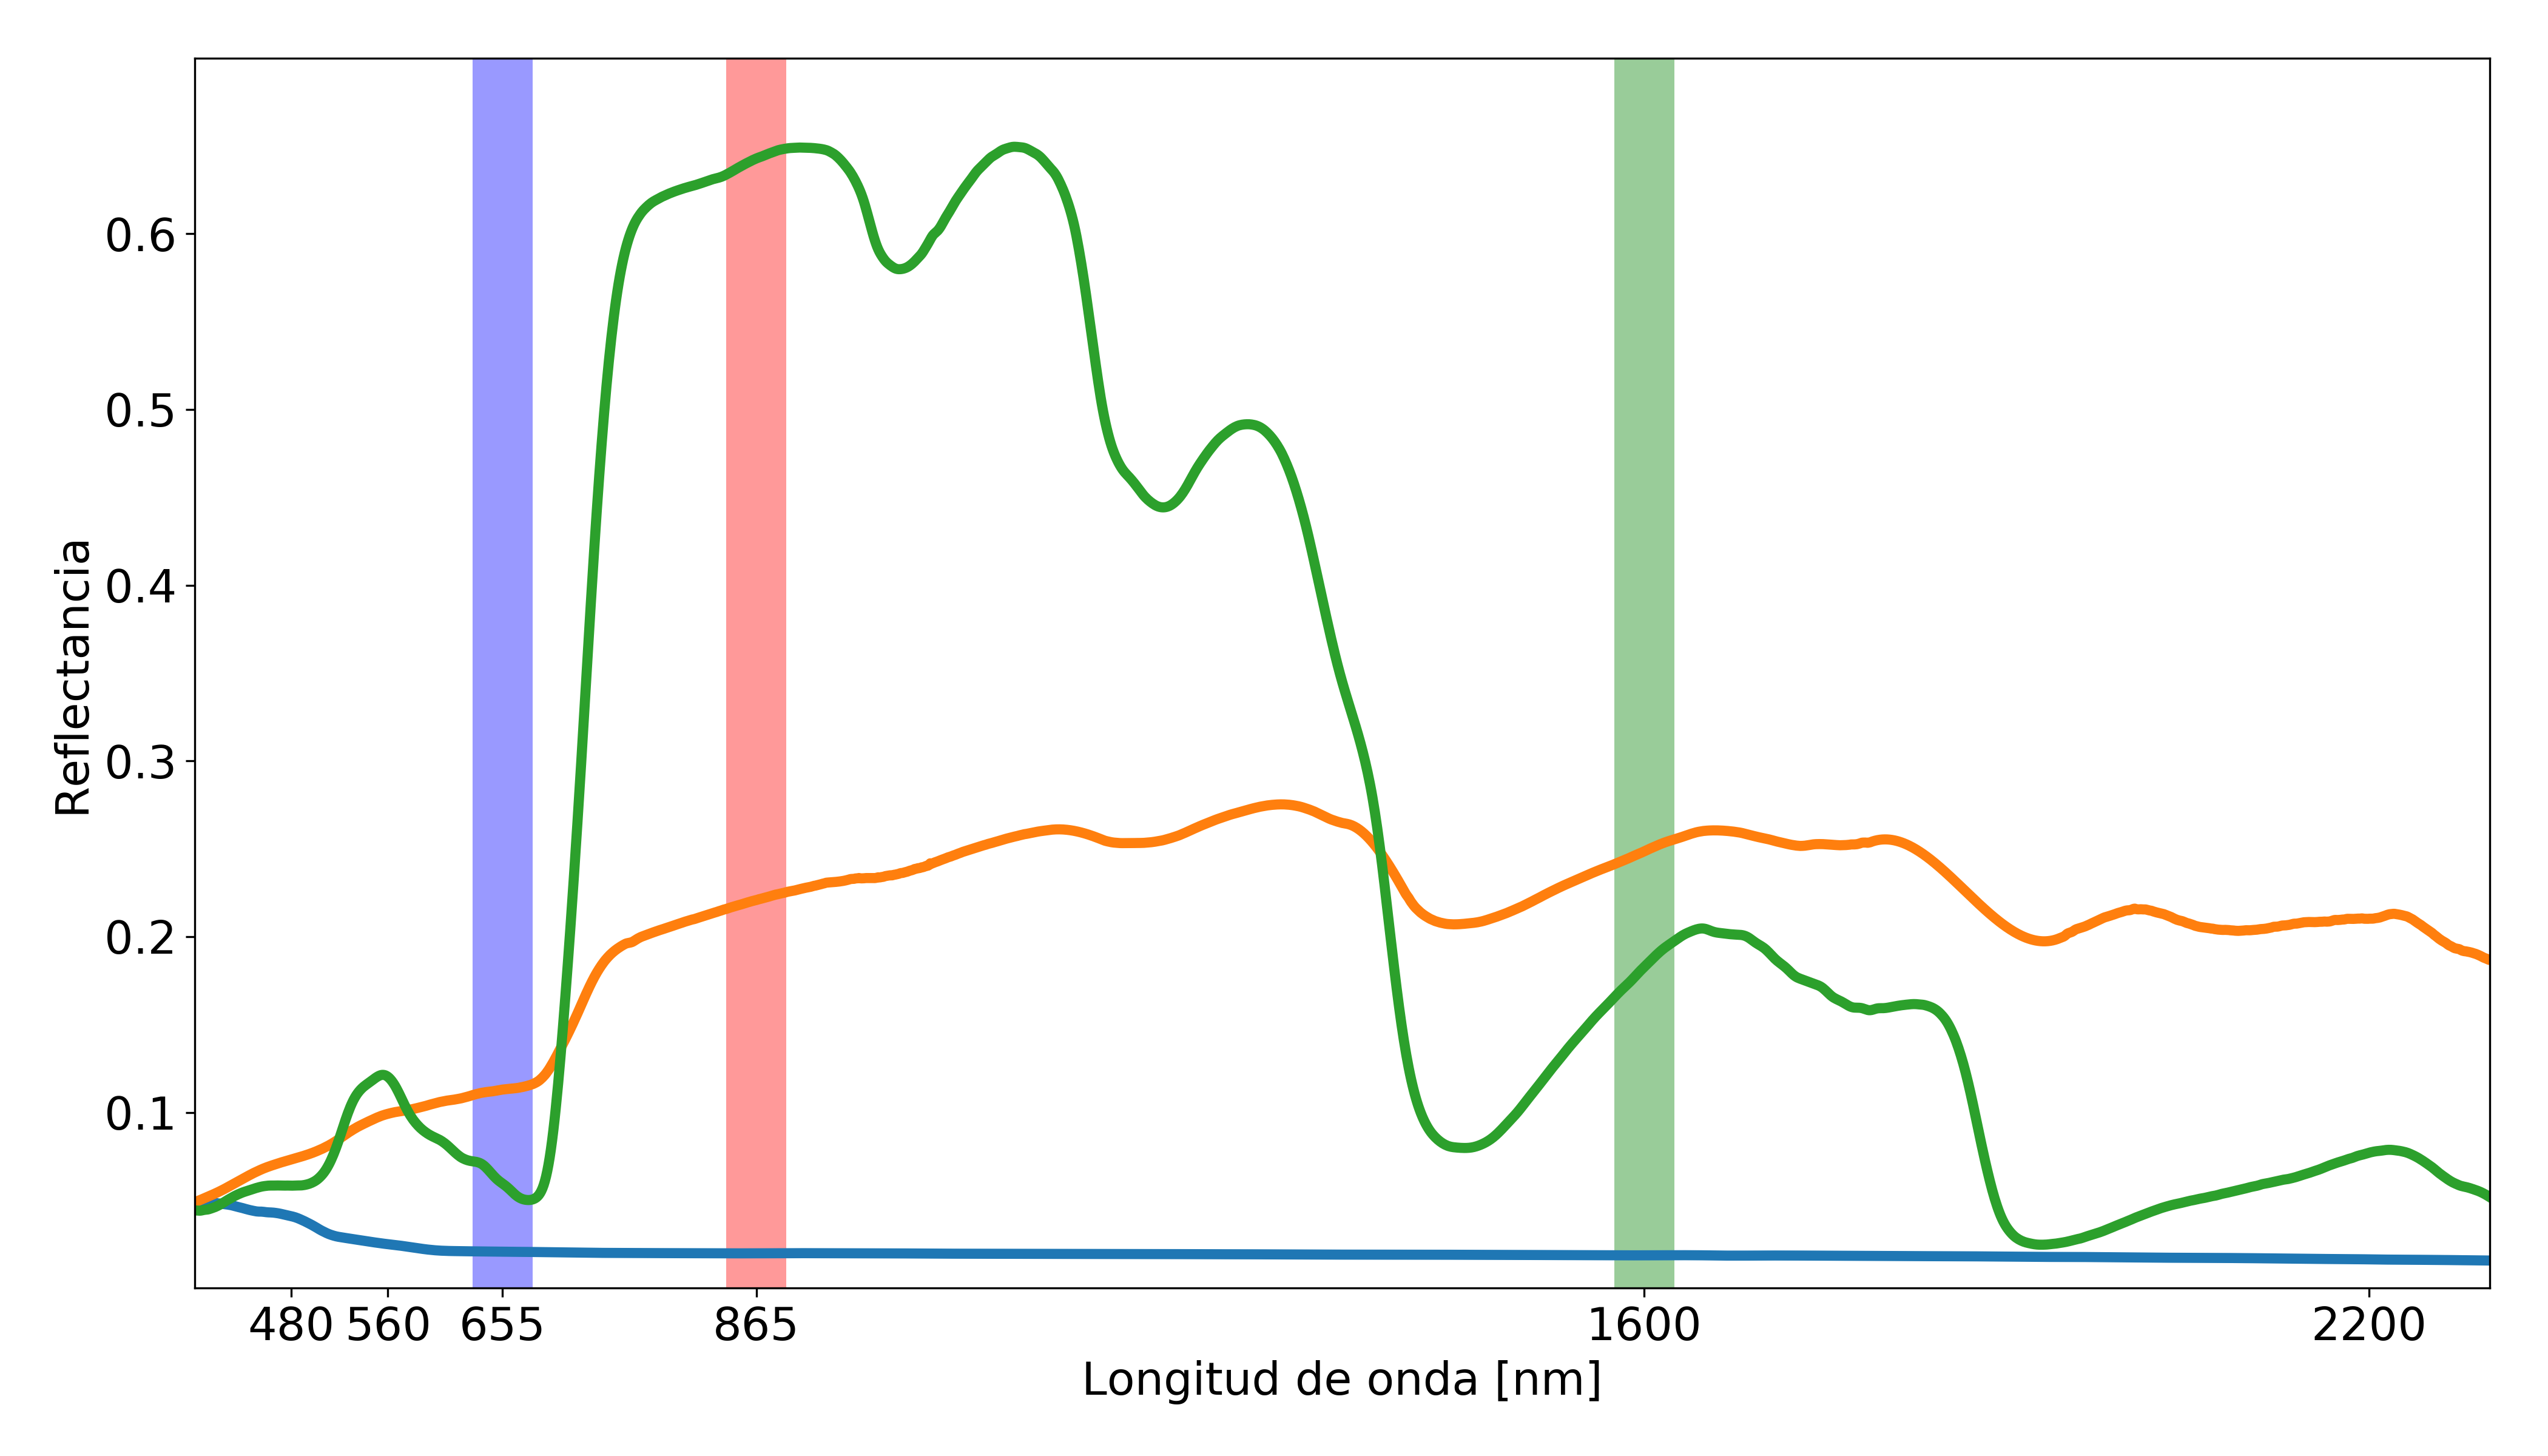
\includegraphics[width=0.8\textwidth]{fig:escomp.png}
    \caption{Interpretación visual - falso color compuesto.}
    \label{}
  \end{figure}
\end{frame}
%--- Next Frame ---%

\begin{frame}{\secname : \subsecname}
  \begin{figure}
    \centering
    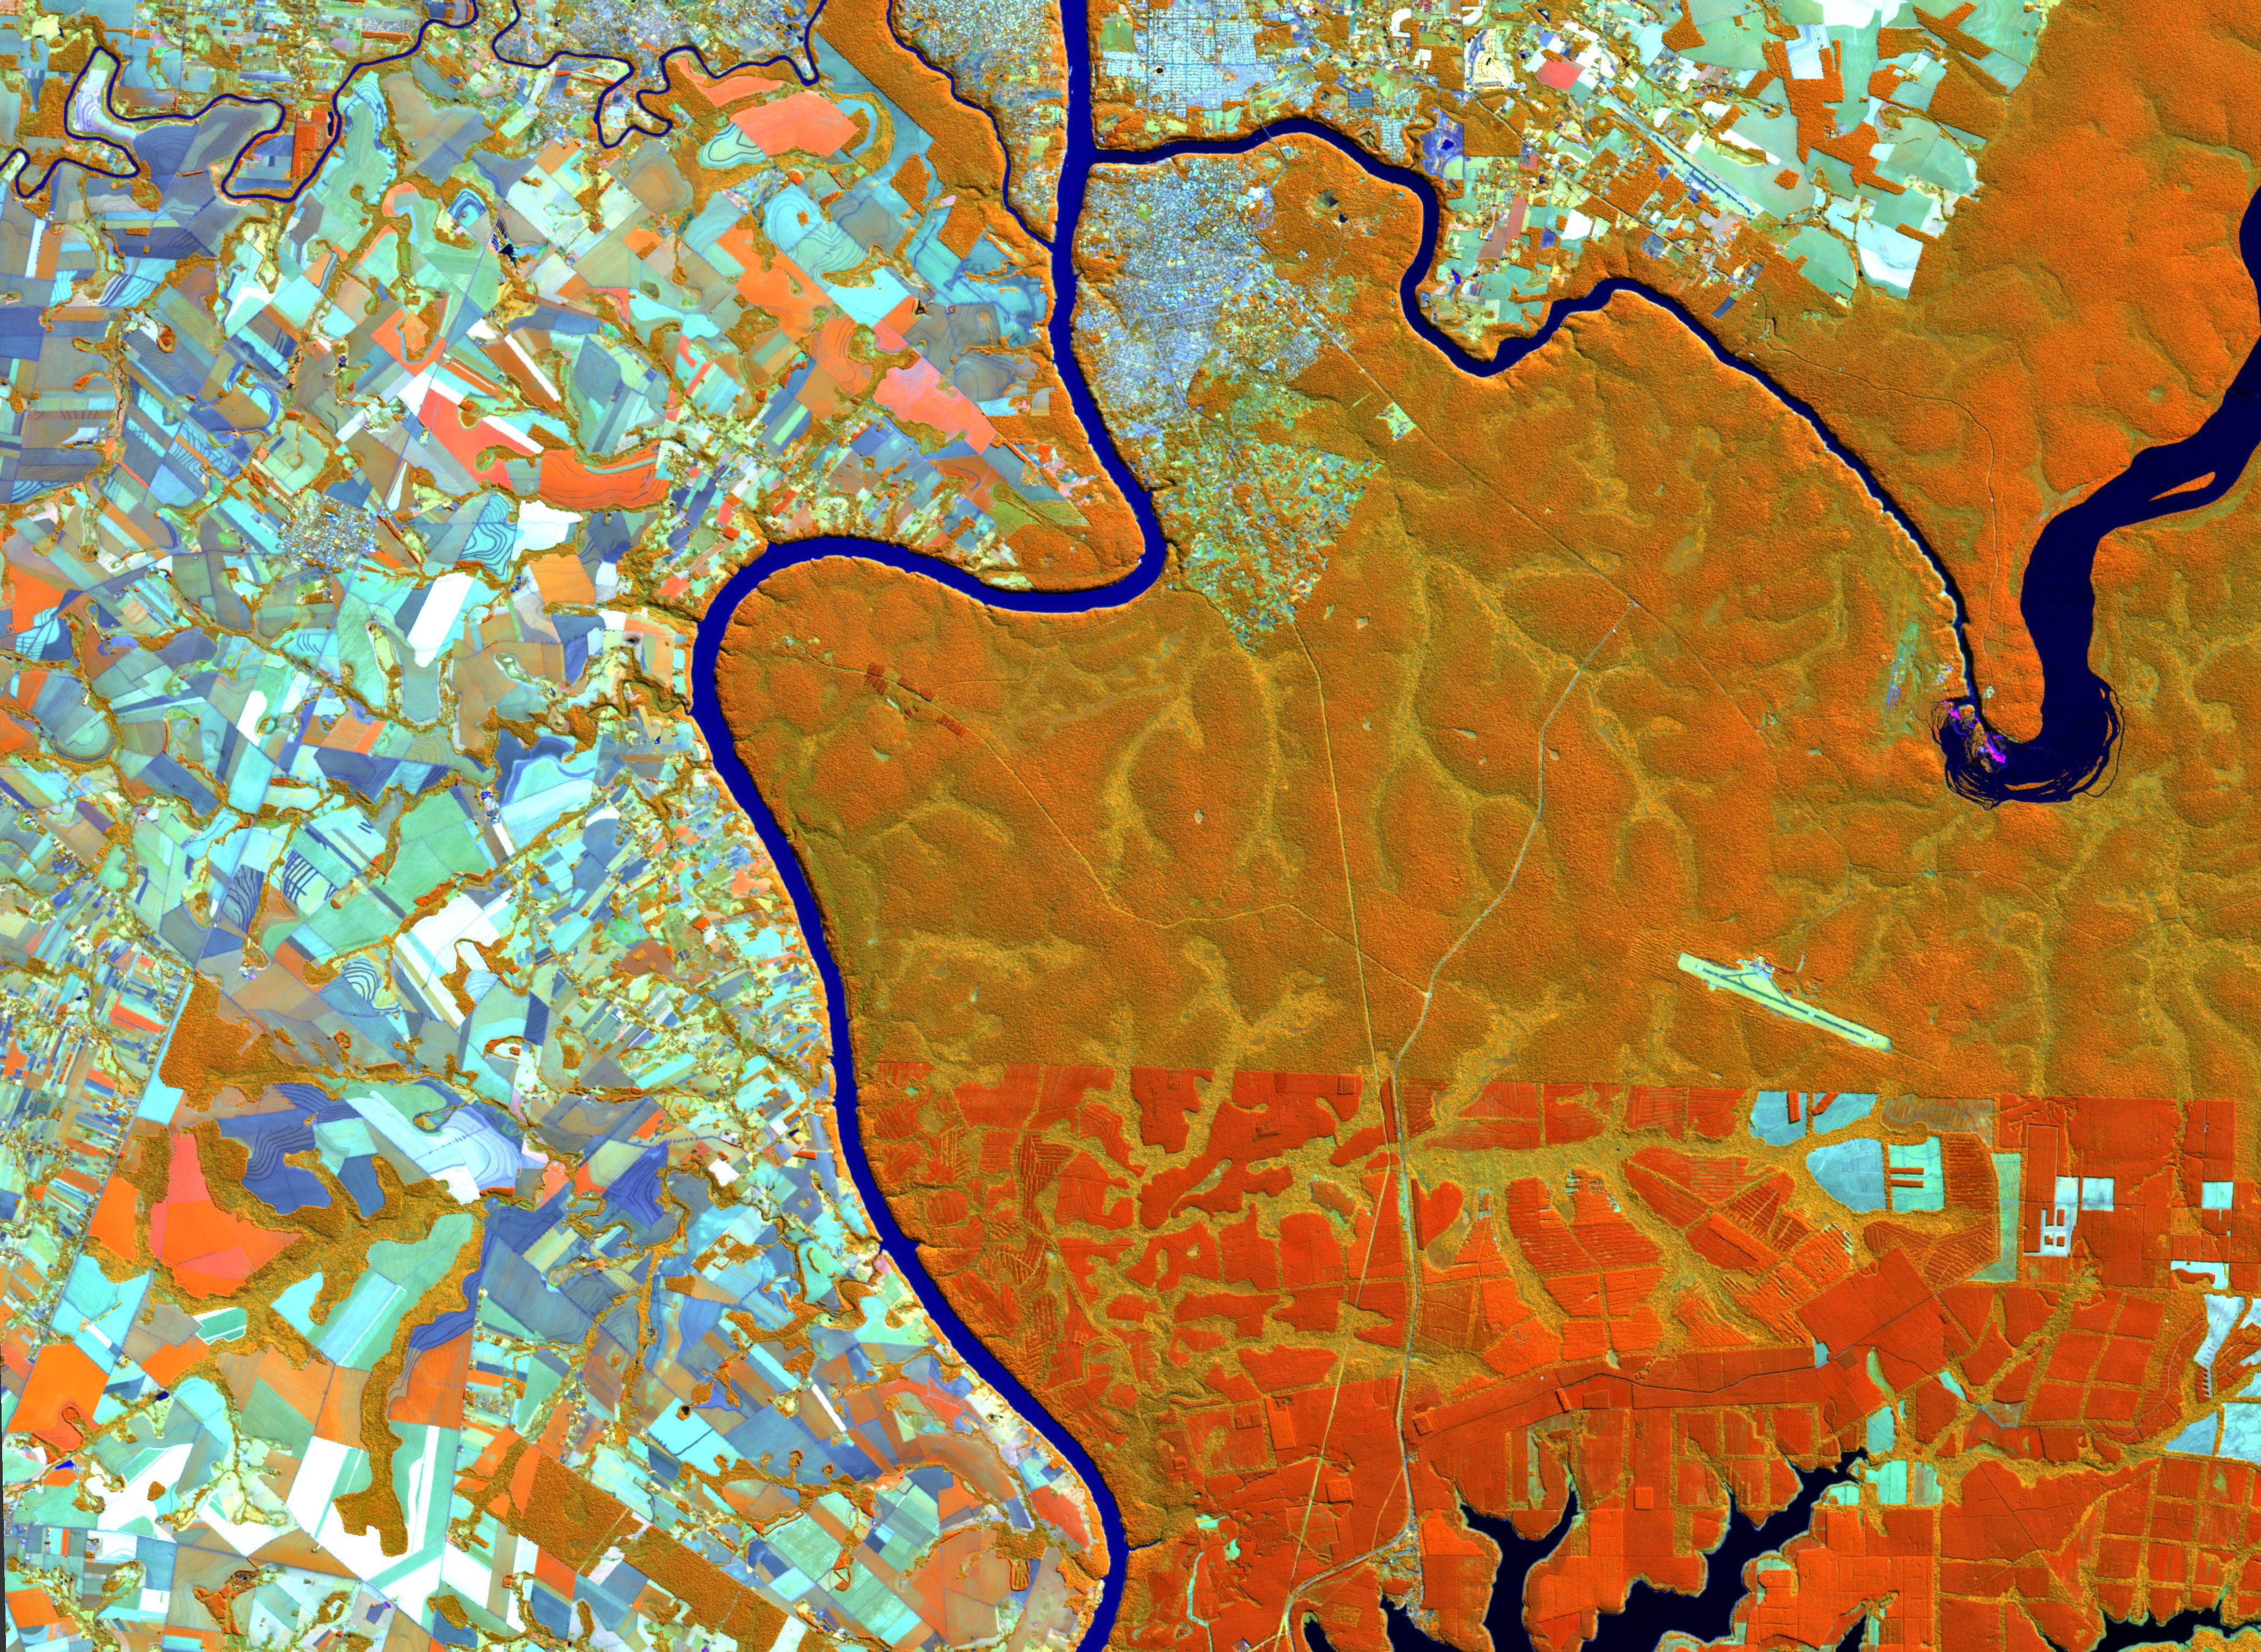
\includegraphics[width=0.6\textwidth]{fig:imcomp.jpeg}
    \caption{Interpretación visual - falso color compuesto.}
    \label{}
  \end{figure}
\end{frame}
%--- Next Frame ---%

\begin{frame}{\secname : \subsecname}
Muchas gracias.
\end{frame}
%--- Next Frame ---%
